%% %%%%%%%%%%%%%%%%%%%%%%%%%%%%%%%%%%%%%%%%%%%%%%%%%
%% Template for a conference paper, prepared for the
%% Food and Resource Economics Department - IFAS
%% UNIVERSITY OF FLORIDA
%% %%%%%%%%%%%%%%%%%%%%%%%%%%%%%%%%%%%%%%%%%%%%%%%%%
%% Version 1.0 // November 2019
%% %%%%%%%%%%%%%%%%%%%%%%%%%%%%%%%%%%%%%%%%%%%%%%%%%
%% Ariel Soto-Caro
%%  - asotocaro@ufl.edu
%%  - arielsotocaro@gmail.com
%% %%%%%%%%%%%%%%%%%%%%%%%%%%%%%%%%%%%%%%%%%%%%%%%%%
\documentclass[12pt]{article}
\usepackage{UF_FRED_paper_style}
\documentclass{scrreprt}
\usepackage{color}
\definecolor{lightgray}{rgb}{0.95, 0.95, 0.95}
\definecolor{darkgray}{rgb}{0.4, 0.4, 0.4}
%\definecolor{purple}{rgb}{0.65, 0.12, 0.82}
\definecolor{editorGray}{rgb}{0.95, 0.95, 0.95}
\definecolor{editorOcher}{rgb}{1, 0.5, 0} % #FF7F00 -> rgb(239, 169, 0)
\definecolor{editorGreen}{rgb}{0, 0.5, 0} % #007C00 -> rgb(0, 124, 0)
\definecolor{orange}{rgb}{1,0.45,0.13}		
\definecolor{olive}{rgb}{0.17,0.59,0.20}
\definecolor{brown}{rgb}{0.69,0.31,0.31}
\definecolor{purple}{rgb}{0.38,0.18,0.81}
\definecolor{lightblue}{rgb}{0.1,0.57,0.7}
\definecolor{lightred}{rgb}{1,0.4,0.5}
\usepackage{upquote}
\usepackage{listings}
% CSS
\lstdefinelanguage{CSS}{
  keywords={color,background-image:,margin,padding,font,weight,display,position,top,left,right,bottom,list,style,border,size,white,space,min,width, transition:, transform:, transition-property, transition-duration, transition-timing-function},	
  sensitive=true,
  morecomment=[l]{//},
  morecomment=[s]{/*}{*/},
  morestring=[b]',
  morestring=[b]",
  alsoletter={:},
  alsodigit={-}
}

% JavaScript
\lstdefinelanguage{JavaScript}{
  morekeywords={typeof, new, true, false, catch, function, return, null, catch, switch, var, if, in, while, do, else, case, break},
  morecomment=[s]{/*}{*/},
  morecomment=[l]//,
  morestring=[b]",
  morestring=[b]'
}

\lstdefinelanguage{HTML5}{
  language=html,
  sensitive=true,	
  alsoletter={<>=-},	
  morecomment=[s]{<!-}{-->},
  tag=[s],
  otherkeywords={
  % General
  >,
  % Standard tags
	<!DOCTYPE,
  </html, <html, <head, <title, </title, <style, </style, <link, </head, <meta, />,
	% body
	</body, <body,
	% Divs
	</div, <div, </div>, 
	% Paragraphs
	</p, <p, </p>,
	% scripts
	</script, <script,
  % More tags...
  <canvas, /canvas>, <svg, <rect, <animateTransform, </rect>, </svg>, <video, <source, <iframe, </iframe>, </video>, <image, </image>, <header, </header, <article, </article
  },
  ndkeywords={
  % General
  =,
  % HTML attributes
  charset=, src=, id=, width=, height=, style=, type=, rel=, href=,
  % SVG attributes
  fill=, attributeName=, begin=, dur=, from=, to=, poster=, controls=, x=, y=, repeatCount=, xlink:href=,
  % properties
  margin:, padding:, background-image:, border:, top:, left:, position:, width:, height:, margin-top:, margin-bottom:, font-size:, line-height:,
	% CSS3 properties
  transform:, -moz-transform:, -webkit-transform:,
  animation:, -webkit-animation:,
  transition:,  transition-duration:, transition-property:, transition-timing-function:,
  }
}

\lstdefinestyle{htmlcssjs} {%
  % General design
%  backgroundcolor=\color{editorGray},
  basicstyle={\footnotesize\ttfamily},   
  frame=b,
  % line-numbers
  xleftmargin={0.75cm},
  numbers=left,
  stepnumber=1,
  firstnumber=1,
  numberfirstline=true,	
  % Code design
  identifierstyle=\color{black},
  keywordstyle=\color{blue}\bfseries,
  ndkeywordstyle=\color{editorGreen}\bfseries,
  stringstyle=\color{editorOcher}\ttfamily,
  commentstyle=\color{brown}\ttfamily,
  % Code
  language=HTML5,
  alsolanguage=JavaScript,
  alsodigit={.:;},	
  tabsize=2,
  showtabs=false,
  showspaces=false,
  showstringspaces=false,
  extendedchars=true,
  breaklines=true,
  % German umlauts
  literate=%
  {Ö}{{\"O}}1
  {Ä}{{\"A}}1
  {Ü}{{\"U}}1
  {ß}{{\ss}}1
  {ü}{{\"u}}1
  {ä}{{\"a}}1
  {ö}{{\"o}}1
}
%
\lstdefinestyle{py} {%
language=python,
literate=%
*{0}{{{\color{lightred}0}}}1
{1}{{{\color{lightred}1}}}1
{2}{{{\color{lightred}2}}}1
{3}{{{\color{lightred}3}}}1
{4}{{{\color{lightred}4}}}1
{5}{{{\color{lightred}5}}}1
{6}{{{\color{lightred}6}}}1
{7}{{{\color{lightred}7}}}1
{8}{{{\color{lightred}8}}}1
{9}{{{\color{lightred}9}}}1,
basicstyle=\footnotesize\ttfamily, % Standardschrift
numbers=left,               % Ort der Zeilennummern
%numberstyle=\tiny,          % Stil der Zeilennummern
%stepnumber=2,               % Abstand zwischen den Zeilennummern
numbersep=5pt,              % Abstand der Nummern zum Text
tabsize=4,                  % Groesse von Tabs
extendedchars=true,         %
breaklines=true,            % Zeilen werden Umgebrochen
keywordstyle=\color{blue}\bfseries,
frame=b,
commentstyle=\color{brown}\itshape,
stringstyle=\color{editorOcher}\ttfamily, % Farbe der String
showspaces=false,           % Leerzeichen anzeigen ?
showtabs=false,             % Tabs anzeigen ?
xleftmargin=17pt,
framexleftmargin=17pt,
framexrightmargin=5pt,
framexbottommargin=4pt,
%backgroundcolor=\color{lightgray},
showstringspaces=false,      % Leerzeichen in Strings anzeigen ?
}%
%
\doublespacing

\setlength{\droptitle}{-5em} %% Don't touch

% %%%%%%%%%%%%%%%%%%%%%%%%%%%%%%%%%%%%%%%%%%%%%%%%%%%%%%%%%%
% SET THE TITLE
% %%%%%%%%%%%%%%%%%%%%%%%%%%%%%%%%%%%%%%%%%%%%%%%%%%%%%%%%%%

% TITLE:
\title{Software Engineering Final Project Report: Car Price Estimator Web Application
}

% AUTHORS:
\author{Juan Cisneros\\% Name author
    \href{mailto:firstauthor@ufl.edu}{} %% Email author 1 
\and Angel Meraz Payan\\% Name author
    \href{mailto:secondauthor@ufl.edu}{} %% Email author 2
\and Luis Perez\\% Name author
    \href{mailto:thirdauthor@ufl.edu}{}%% Email author 3
%\and Forth Author\\% Name author
%    \href{mailto:forthuthor@ufl.edu}{\texttt{forthuthor@ufl.edu}}%% Email author 4
    }
    
% DATE:
\date{\today}

% %%%%%%%%%%%%%%%%%%%%%%%%%%%%%%%%%%%%%%%%%%%%%%%%%%%%%%%%%%
% %%%%%%%%%%%%%%%%%%%%%%%%%%%%%%%%%%%%%%%%%%%%%%%%%%%%%%%%%%
\doublespacing
\begin{document}
% %%%%%%%%%%%%%%%%%%%%%%%%%%%%%%%%%%%%%%%%%%%%%%%%%%%%%%%%%%
% %%%%%%%%%%%%%%%%%%%%%%%%%%%%%%%%%%%%%%%%%%%%%%%%%%%%%%%%%%
% ABSTRACT
% %%%%%%%%%%%%%%%%%%%%%%%%%%%%%%%%%%%%%%%%%%%%%%%%%%%%%%%%%%
% %%%%%%%%%%%%%%%%%%%%%%%%%%%%%%%%%%%%%%%%%%%%%%%%%%%%%%%%%%
{\setstretch{.8}
\maketitle
% %%%%%%%%%%%%%%%%%%
\begin{abstract}
% CONTENT OF ABS HERE--------------------------------------
In this final project for software engineering, we utilize various technologies and use our acquired knowledge to design, implement and deploy a web application. The application is created using JavaScript, HTML, and CSS, with a JSON storage bin acting as our database. In this paper, we describe the process and work put in by the team to complete the project from the design phase to deployment. 

% END CONTENT ABS------------------------------------------
\noindent
\textit{\textbf{Keywords: }%
Software Engineering; Web Application;.} \\ %% <-- Keywords HERE!
\noindent
\end{abstract}
}

% %%%%%%%%%%%%%%%%%%%%%%%%%%%%%%%%%%%%%%%%%%%%%%%%%%%%%%%%%%
% %%%%%%%%%%%%%%%%%%%%%%%%%%%%%%%%%%%%%%%%%%%%%%%%%%%%%%%%%%
% BODY OF THE DOCUMENT
% %%%%%%%%%%%%%%%%%%%%%%%%%%%%%%%%%%%%%%%%%%%%%%%%%%%%%%%%%%
% %%%%%%%%%%%%%%%%%%%%%%%%%%%%%%%%%%%%%%%%%%%%%%%%%%%%%%%%%%

% --------------------
\section{Introduction}
% --------------------

Software engineering is the process of creating software systems, software engineering has a set of processes on how to develop software. We begin with an idea for a product that will serve a customer or provide certain functionality to benefit or improve a process in a company or organization. Our idea was to create an application of some sort that would estimate the prices of a vehicle based on certain criteria which we would obtain as input from a user. We also discussed making our project open-source since some of the tools and technologies we would be using are also open-source, we decided to use the MIT License for our project \cite{MIT}. This application should follow a logical and smooth flow because it will work depending on provided options that we obtain from the user. In order for this website to be fully functional we must implement a user interface that is uniform and will assist the user in choosing the options or suggestions that they desire. The results shall be displayed on the web page and it will have condensed information and the different attributes that made the price of the vehicle result in whatever the outcome was. 




\begin{figure}[H]
\caption{Technologies, and Languages}
\centering
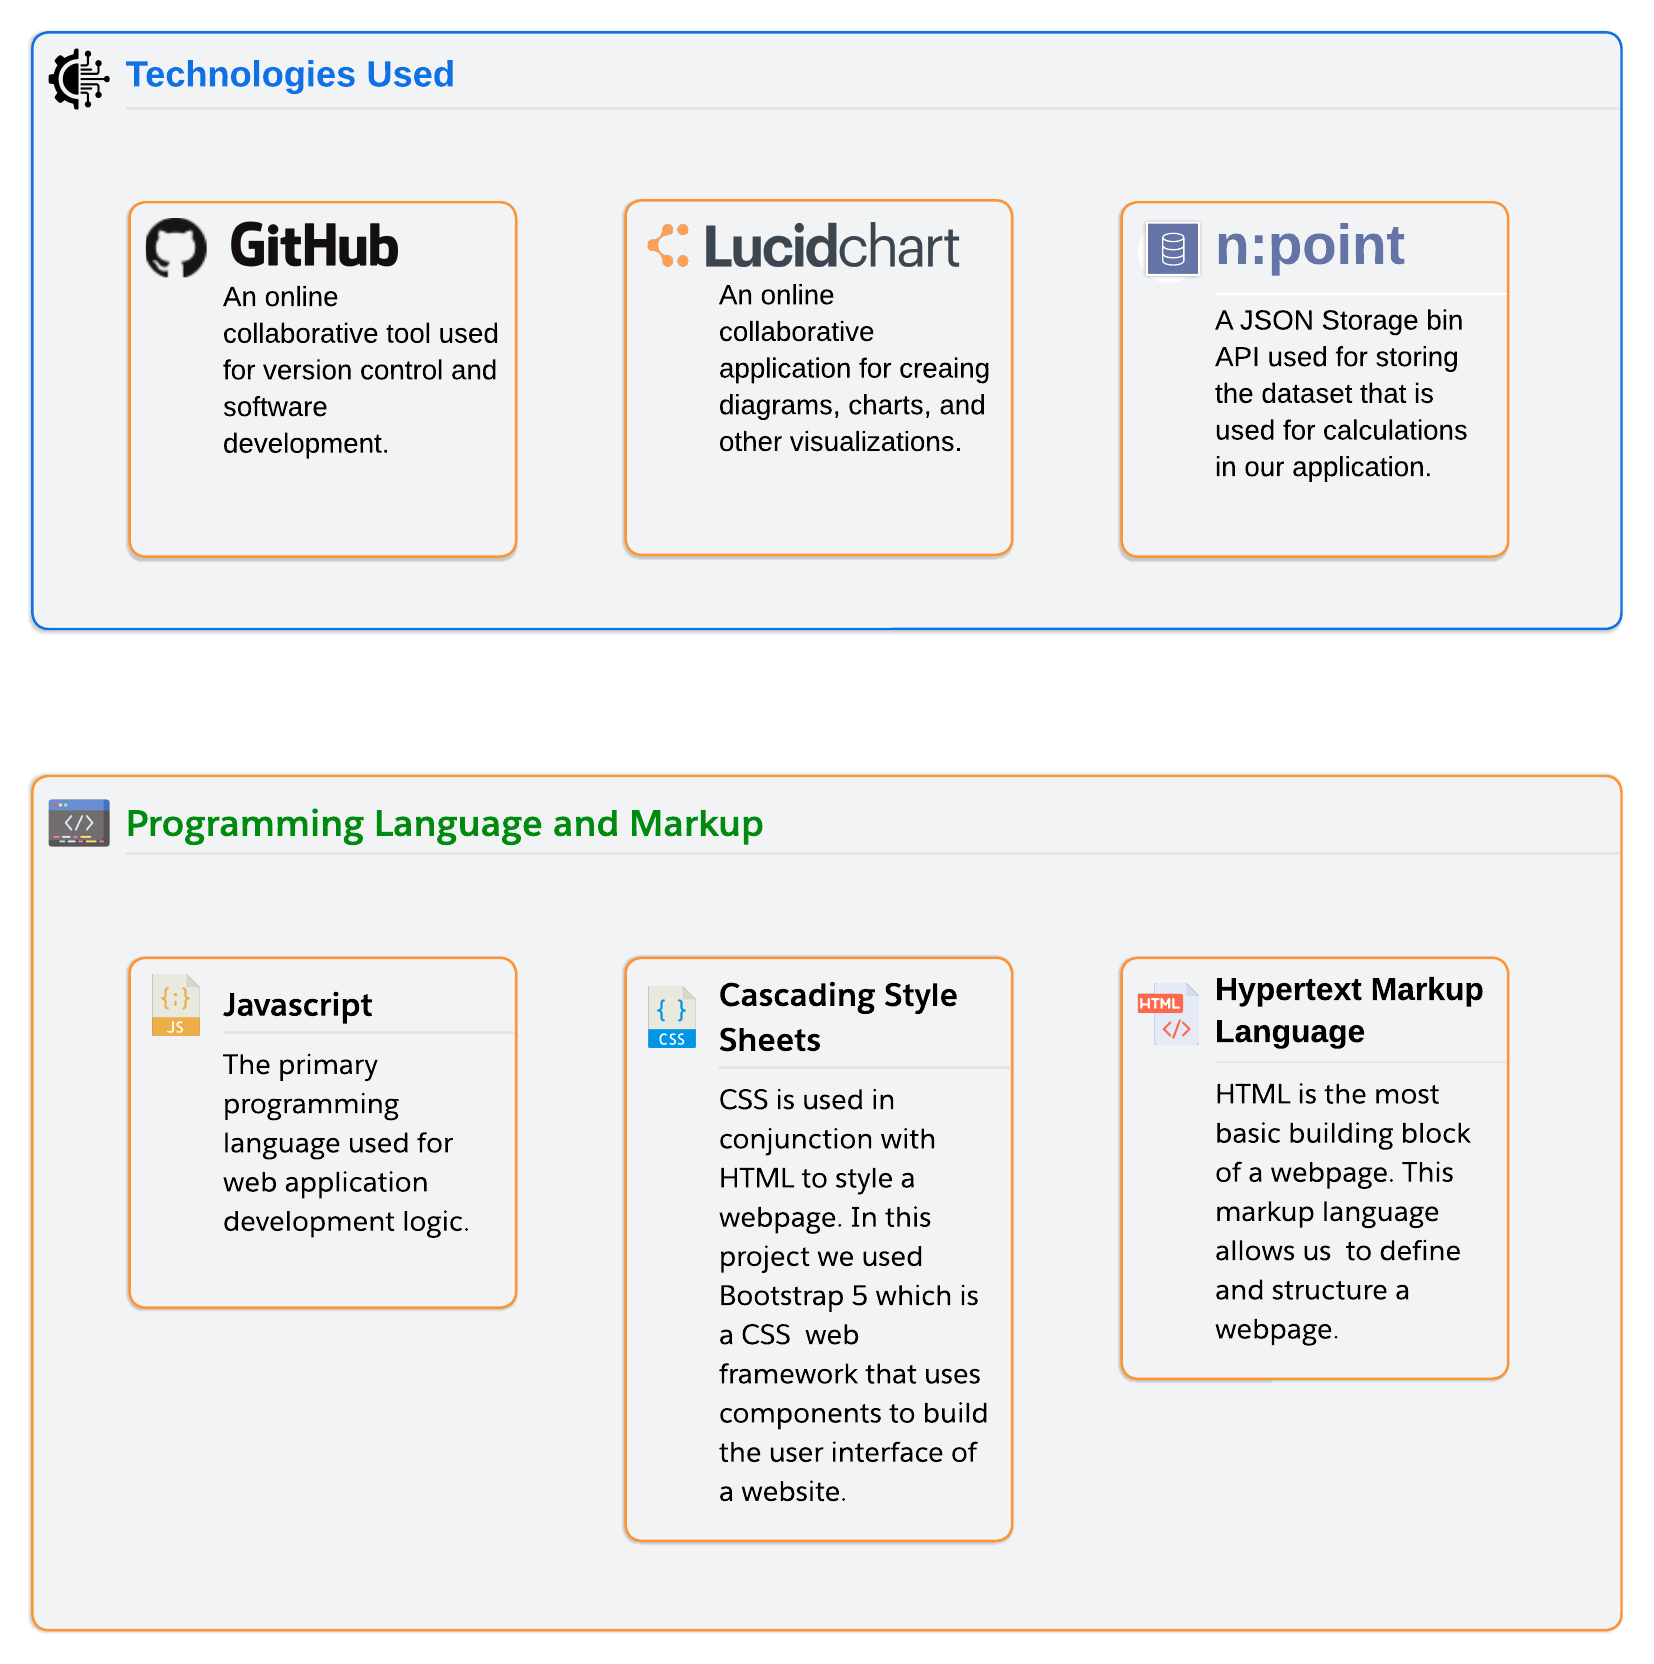
\includegraphics[scale=.25]{figures/Technologies Used.png}\\
\end{figure}
\noindent We now discuss the technologies we used for our development process. Figure 1 showcases the technologies and tools we utilized for this project. We decided to use GitHub for development and source control, this tool was an essential piece in keeping our program well-documented and made it easier for us to make contributions to the project. GitHub also has a feature called GitHub pages that allows us to host static websites, our application could be constructed as a static website that runs on the client side. Another crucial tool is Lucidchart which is an online collaborative web application that allowed us to create diagrams and other visualizations. This tool allowed us to create many of the diagrams used for designing our application and also accompanying the visual aids for our report and presentation. The final but also highly important technology we used was the free and open-source JSON storage bin API n:point\cite{npoint.io}. This tool essentially acted as our data storage, this storage stores a JSON array that contains the data set that will be used for calculating prices in our application. The n:point API works in conjunction with JavaScript FETCH API \cite{APIs} to retrieve the JSON array from the online hosted storage bin that contains our data. Again since our application is meant to run on the web browser the languages and markup we would be using to construct our website are the commonly used technologies of JavaScript, HTML, and CSS. For JavaScript, we would be using the core "Vanilla" JavaScript \cite{JS} version meaning without any external libraries such as JQuery or JavaScript frameworks such as React Native, instead, we used built-in tools and libraries such as the FETCH API\cite{web}. In terms of HTML \cite{HTML} and CSS \cite{CSS}, we decided to use Bootstrap 5 which is a free and open-source HTML and CSS framework that consists of reusable components\cite{thornton_otto}. This framework provides pre-built reusable components which makes developing the UI (user interface) much faster with properly documented code. Bootstrap 5 is also used for building responsive web pages that automatically conform all content of a web page to the size of the device accessing the web page. This is an important feature of this framework since it means we do not have to create a separate website specifically for mobile devices, allowing us to same development time. 

% --------------------
\section{Methodology}
% --------------------

\subsection{Requirements and definitions and System and Software design}                   
 The first key step in the development process is deciding the development methodology to use for developing our web application. As a group, we discussed the various approaches to the development process of our application, and what stood out most was the waterfall methodology \cite{waseem_2022}. The waterfall method is comprised of the flowing steps: first, we create system requirements and documentation, then we design the system (this includes creating flowcharts and diagrams, and brainstorming technologies to use), next we implement the system based on the requirements and design patterns, finally we test the application and perform reevaluations to ensure the product is ready to be released, finally we deliver the finished application (this step means we deploy the application so that it is accessible by the user), and finally we maintain the project after delivery to fix errors or to add extra functionally. As we can see in Figure 2 we start with system requirements and definitions. We note that our system requirements were updated twice so we will only discuss our most recent updated requirements. 

\begin{figure}[H]
\caption{Waterfall methodology for software development}
\centering
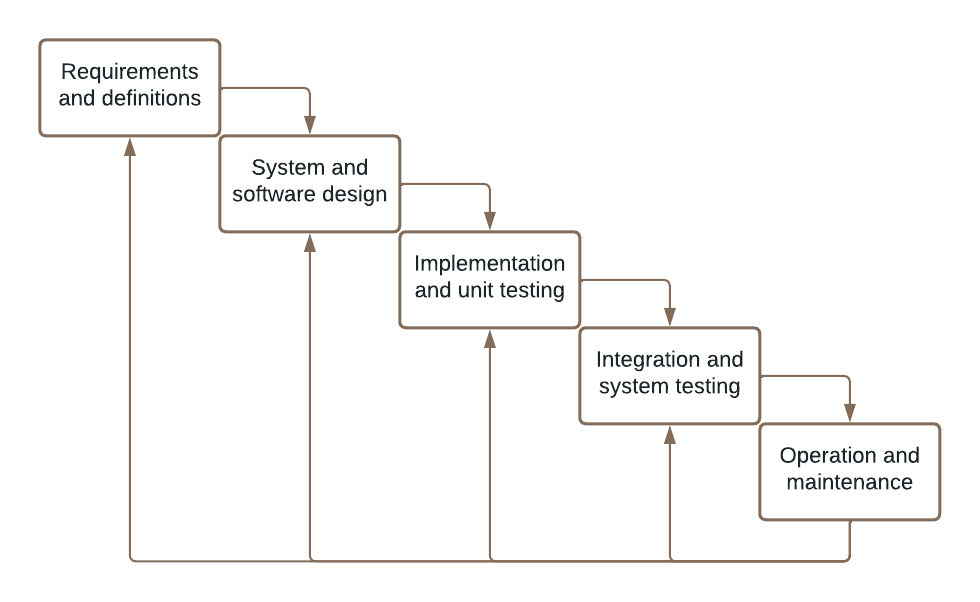
\includegraphics[scale=.45]{figures/Waterfall Methodology.png}\\
\end{figure}
\noindent Our system requirements were created by us but will simulate a client doing business with our team, in essence, the client wants us to develop a web application based on these requirements (Reference Appendix \ref{subsec:A} for these requirements). The first section of requirements basically states what we are building, first, it must be a website, this requires the use of a web browser, and as previously stated this will work on any desktop and mobile device of any operating system that supports the internet connection and web browsing. This section also states some behavior that the application should have such as providing navigation and how the user experience should act. The next section describes how the home page should function the main purpose of this web page is to inform the user about the application. The next section goes more into detail on how the application that estimates the price of a vehicle should function. After we discussed these requirements we were ready to begin system and software design, in this stage we created flow charts and diagrams of how the web application would be implemented. Figure 3 visualizes the description of the first set of requirements for how the application will be accessed by a user. 

\begin{figure}[H]
\caption{Accessing Application Diagram}
\centering
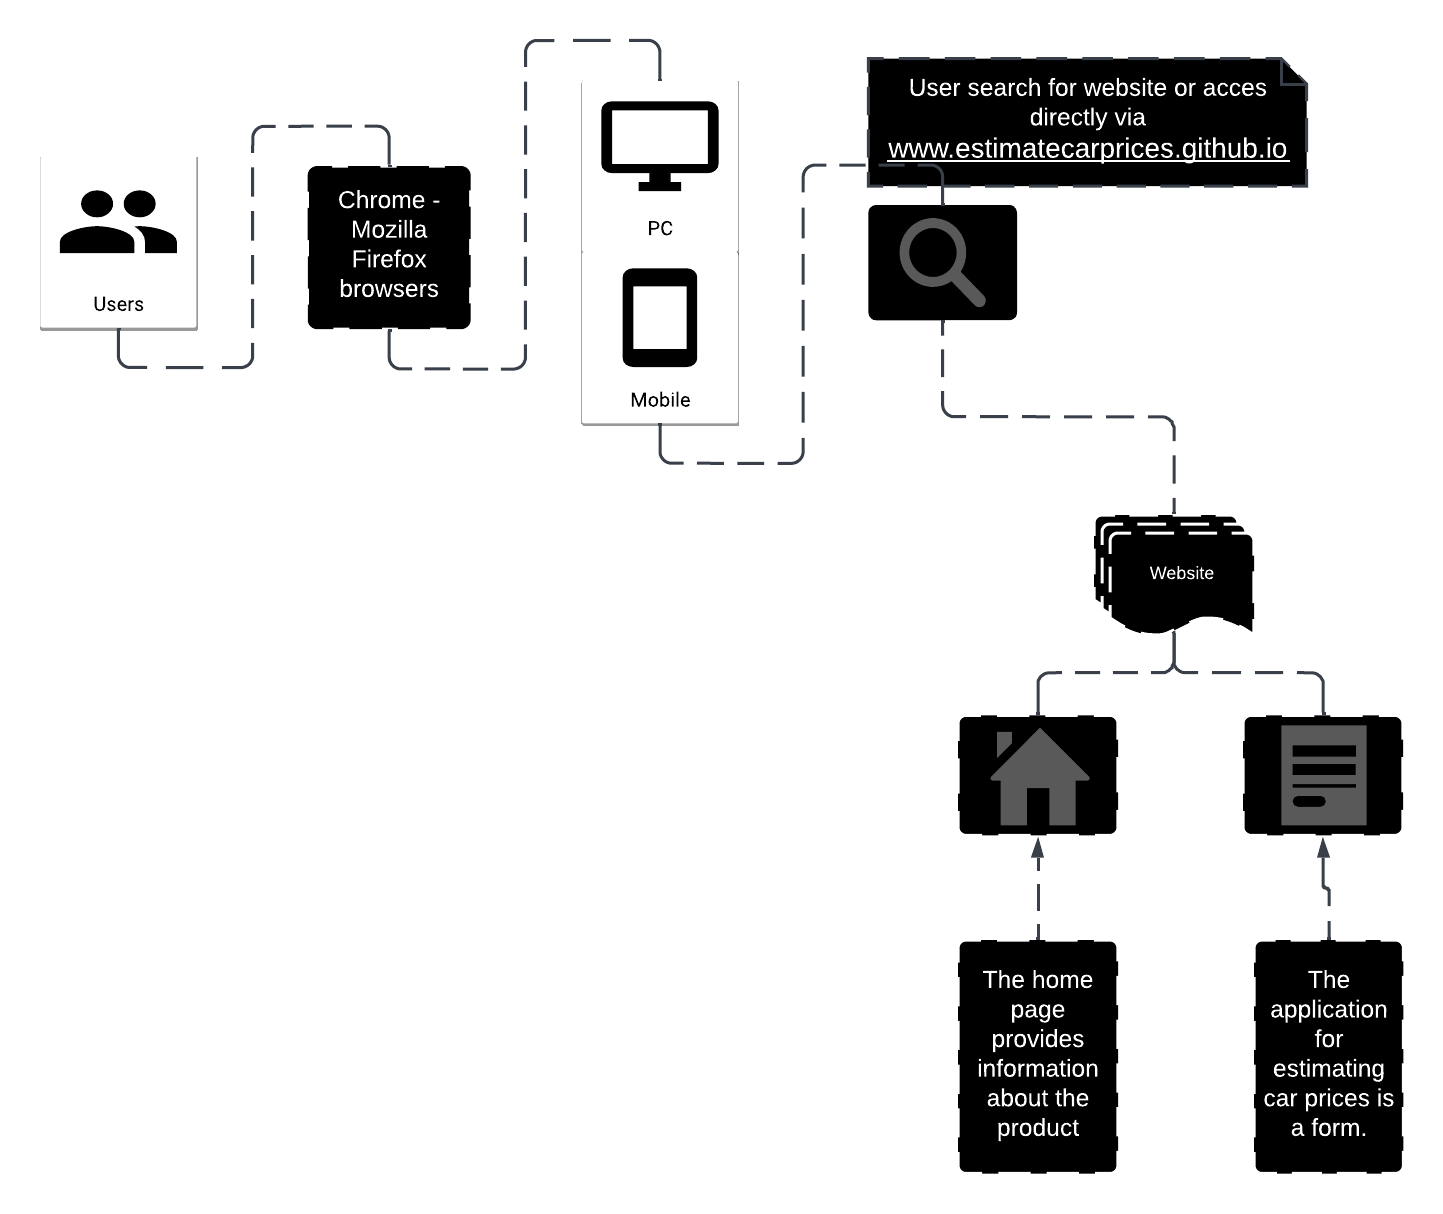
\includegraphics[scale=.3]{figures/Accessing Application Flowchart.png}\\
\end{figure}
\noindent As described by Figure 3 the user will access a web browser using either a mobile device or a Laptop or a Desktop PC, the user will then directly access the website using the URL shown or via a search engine query. Accessing the website will start out with the user seeing the home page and at any point, the user can access the price estimating application via the navigation bar. The next figure describes the structure of what the home web page or the landing page will look like.

\begin{figure}[H]
\caption{Homepage or Landing Page Structure}
\centering
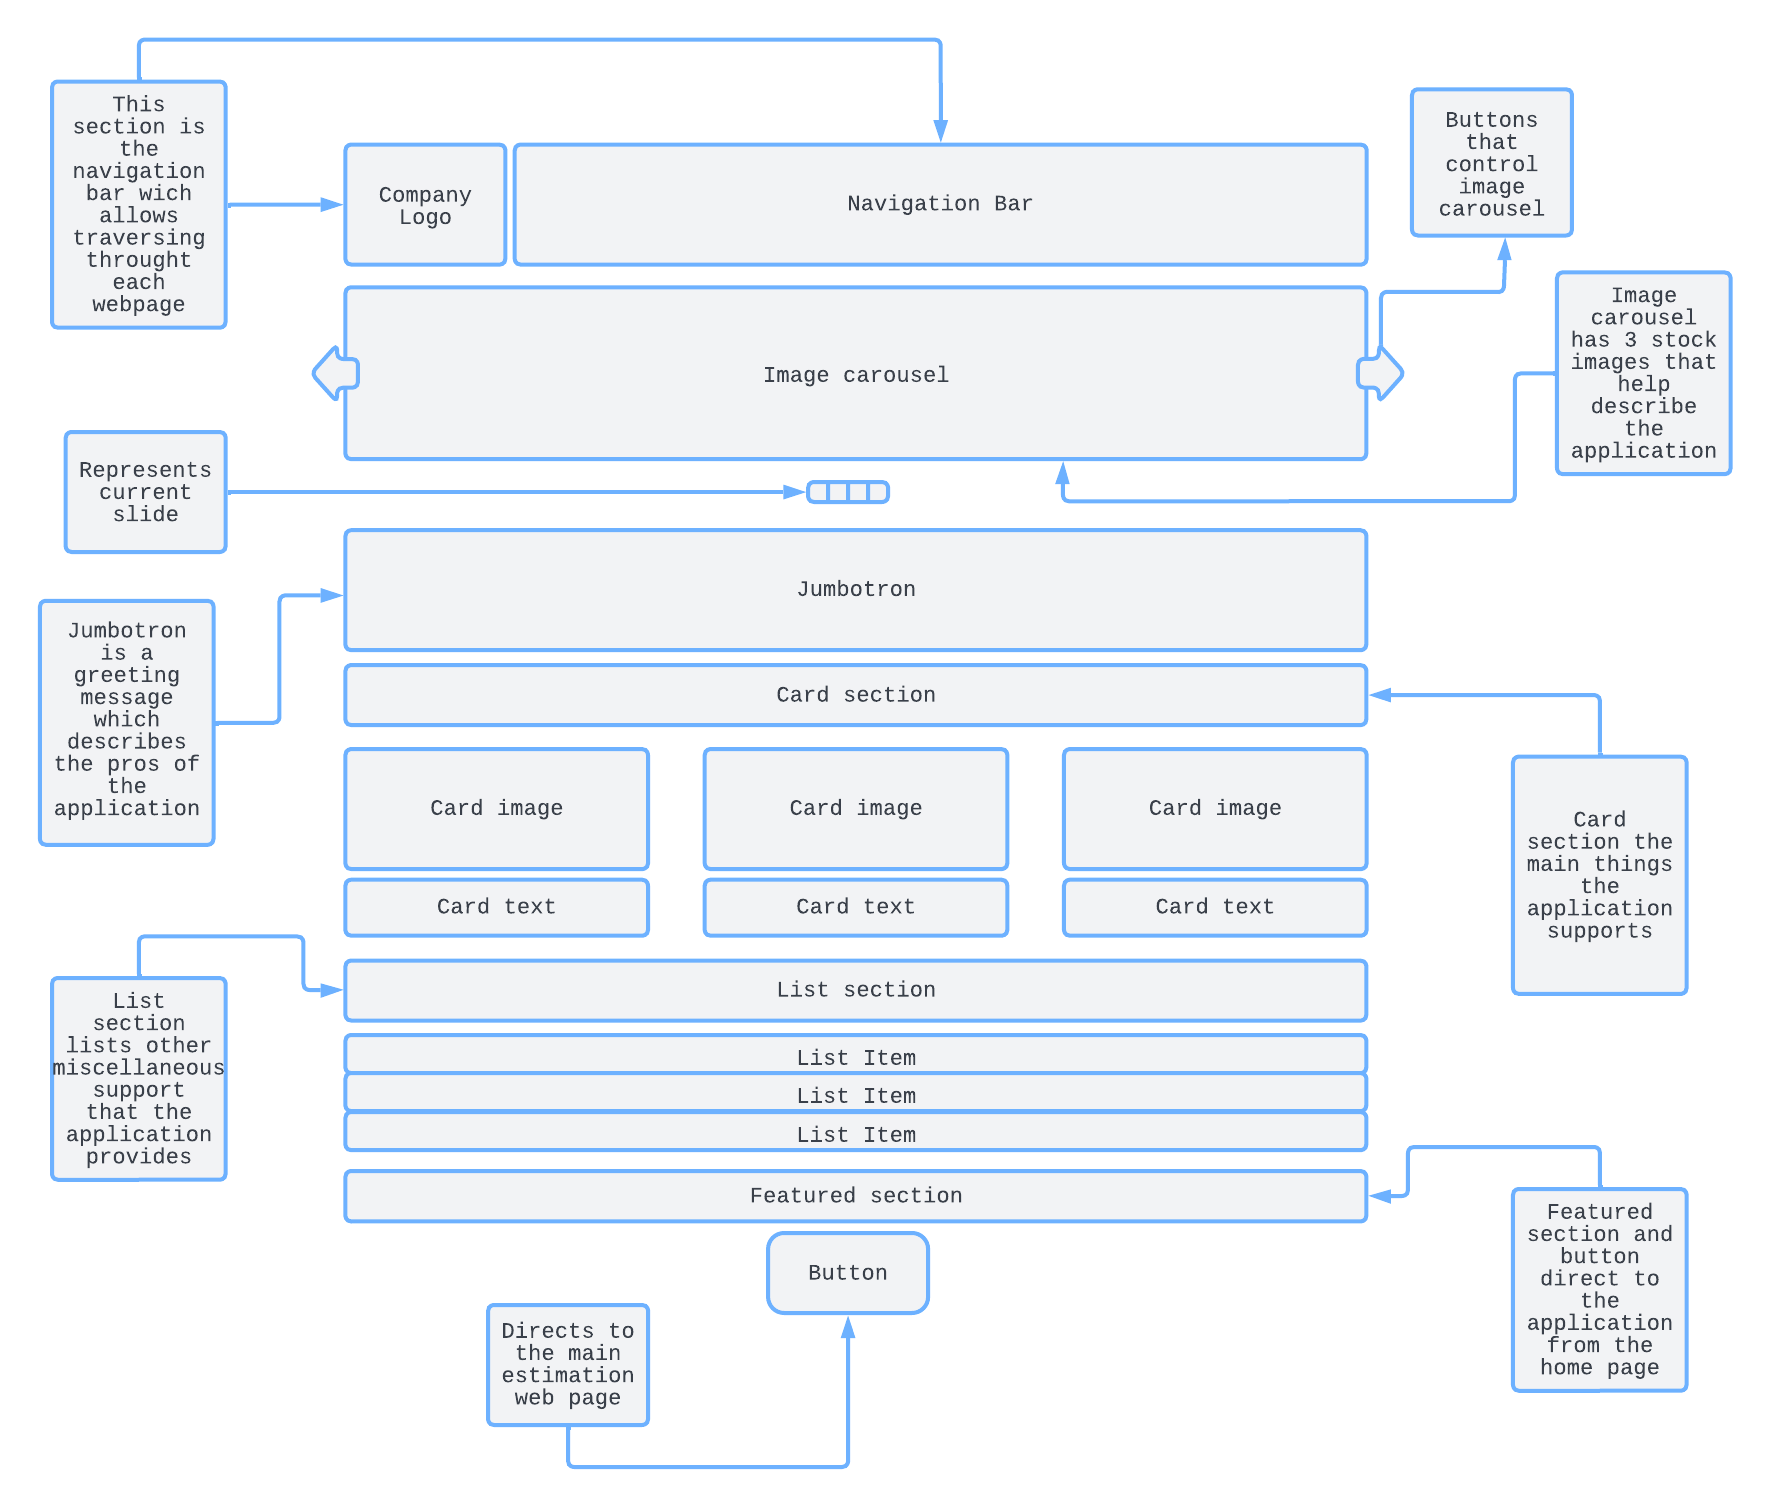
\includegraphics[scale=.26]{figures/Homepage Mockup.png}\\
\end{figure}
\noindent As we can see from Figure 4 the structure of the homepage follows the provided requirements that it must contain a navigation bar, followed by an image carousel then a large section containing information about was is supported by the application. It must also end with a section that contains a button that directs to the estimation web page. It is a convention for the navigation bar to be at the top of a web page since the browser upon loading a web page starts from the very top, so this will allow fast navigation through the website. Again following the principle that the contents of a web page are loaded from the top to bottom we want to catch the user's eye by providing visuals, in this case, we added stock images in a carousel that briefly introduces the user to the application. The jumbotron section provides an actual welcome message to the user, while the card section provides visual imagery of the support provided by the application and the list section reinforces other support provided. The button in the featured section is placed at the bottom of the page to draw in the user to click on the link with leads to the estimation web page. Each section is placed in that specific order to make the web page easy to follow and continuous. A note on the web page structure, for each section such as navigation, image carousel, jumbotron, and so on, we utilized Bootstrap 5 components to build the web page. 

\begin{figure}[H]
\caption{Estimation Web-page Architecture Flow Chart}
\centering
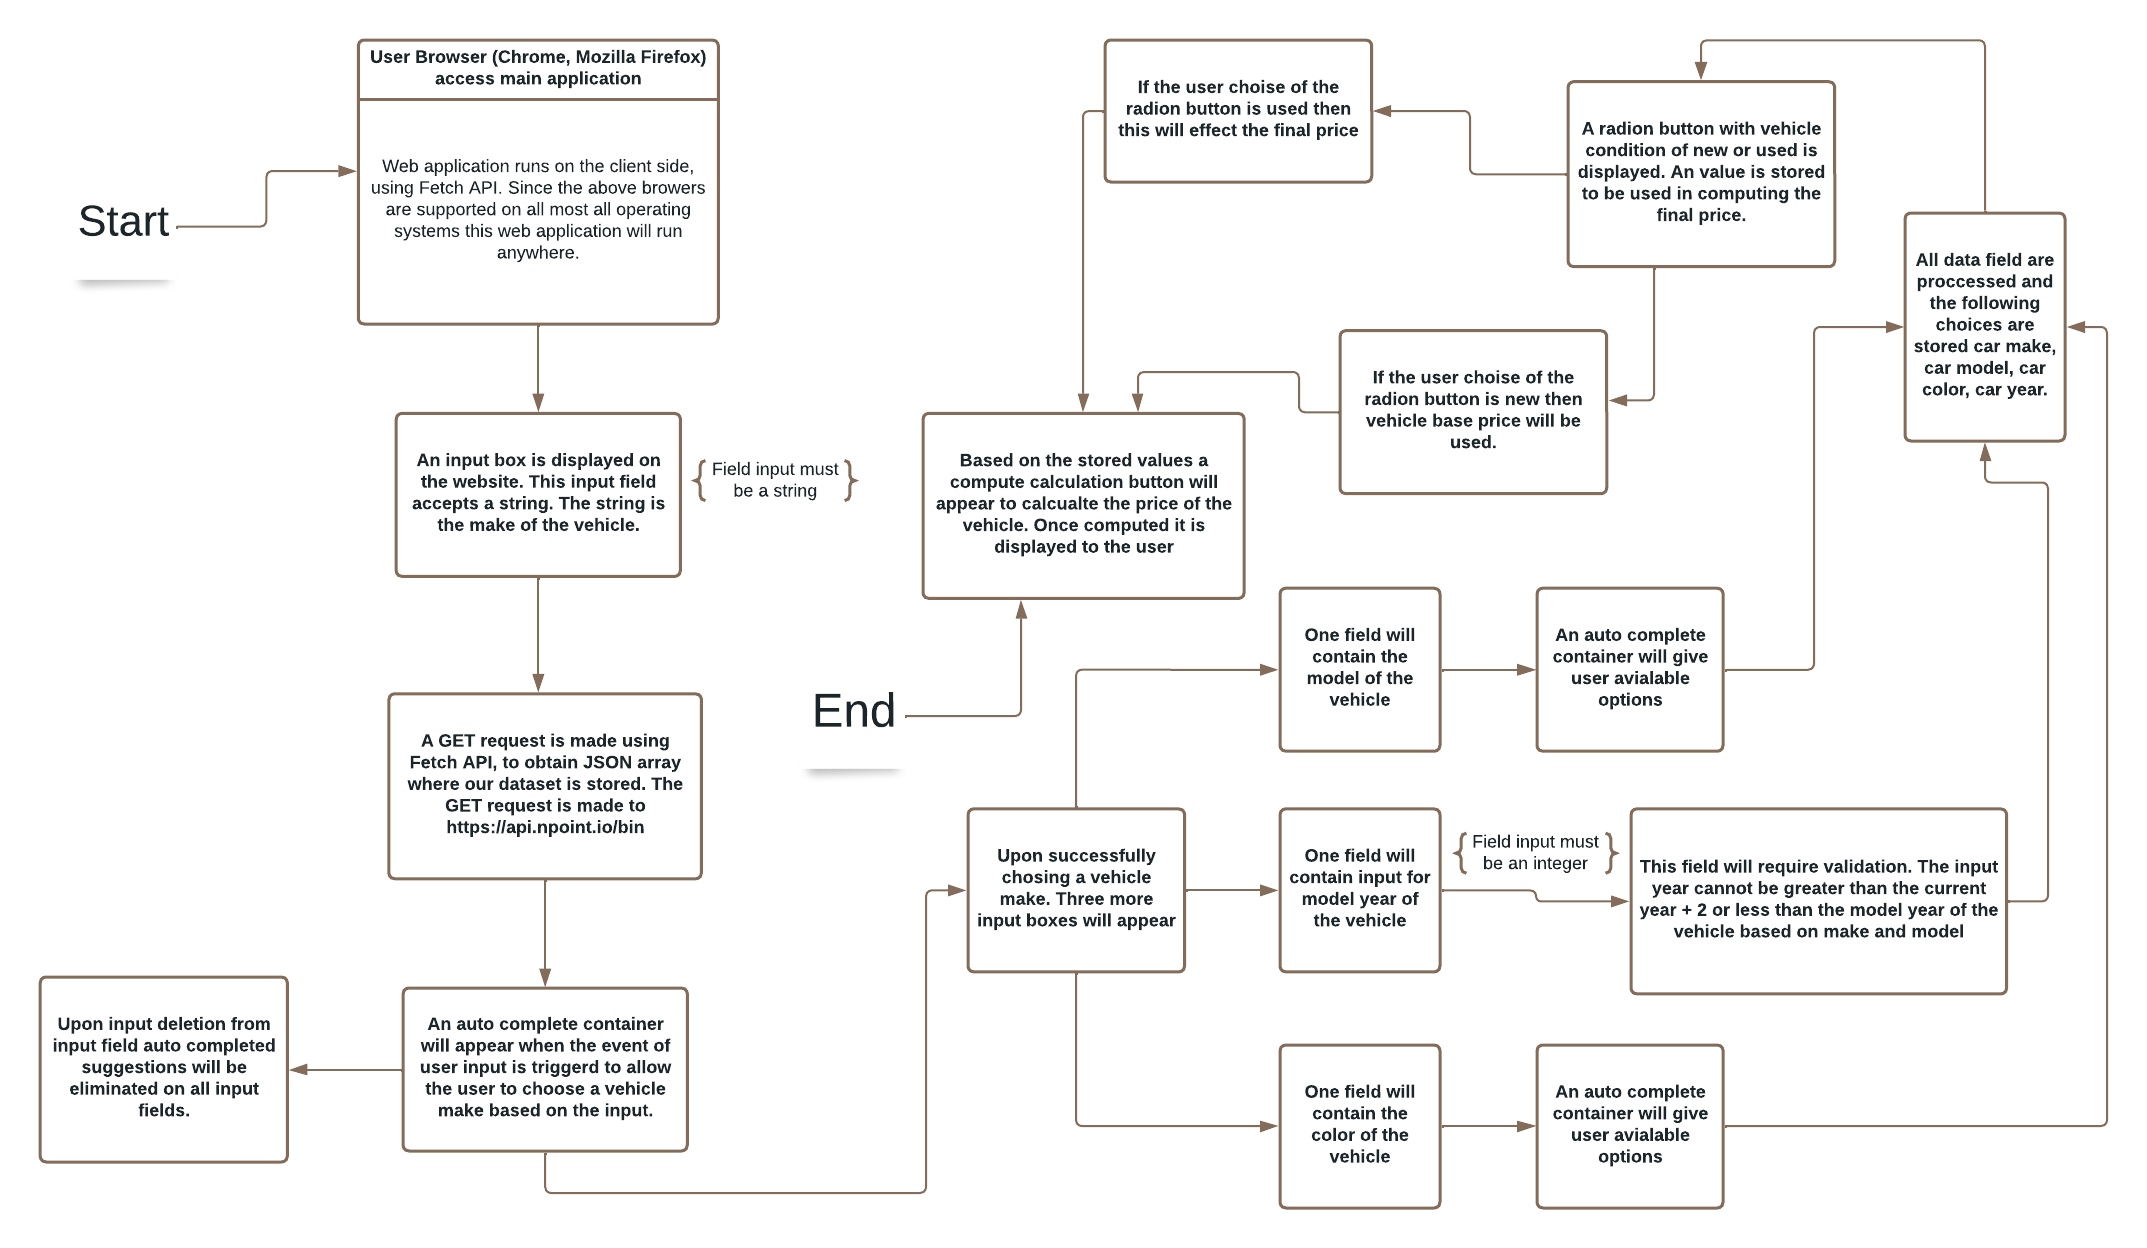
\includegraphics[scale=.22]{figures/Application Architecture.png}\\
\end{figure}

\noindent Figure 5 describes the process flow of the architecture for the estimation web page, while Figure 6 is the flow sequence of what the actual web page will look like and how it will function. The application begins by prompting the user with a form that receives input. This form takes in a string input and makes a GET request using FETCH API to the JSON storage bin to retrieve the data. Then using JavaScript built-in libraries we will match the user input with what is stored in the JSON array data that was fetched to display options, these options are the make of a vehicle more specifically the car make the user is searching for. In essence, this feature is similar to a search menu that provides a user with auto-completed suggestions, so that way there is no need to handle incorrect or irrelevant input by the user in common string input forms. Each option or suggestion based on the input is a clickable button that will store the value of the selected option or suggestion, after a user clicks a certain button all other options or suggestions will be erased until the user decides to change the input on the form. This basic principle is applied to the rest of the forms that take in the input of the vehicle model, and color. For reference on how the process works see Figure 6. 
The section that takes in the year of a vehicle is also a form much like the first, in this case, this form accepts an integer, and we must handle incorrect or irreverent input. The radio button seen in Figure 6 is a type of button that has only one of two states, new or used, this button gets toggled by the user and is used for calculating the estimated price of a vehicle. We note that our design was made to follow procedural programming paradigm along with JavaScript's event-driven programming. This is because after the user triggers one event another event will be set in motion, and there is a logical sequence or procedure for displaying the application to the user. So overall our architecture design was made to have this logical sequence so that a user finds the application intuitive and easy to use.
\begin{figure}[H]
\caption{Estimation Web-page Mock-up Flow Chart}
\centering
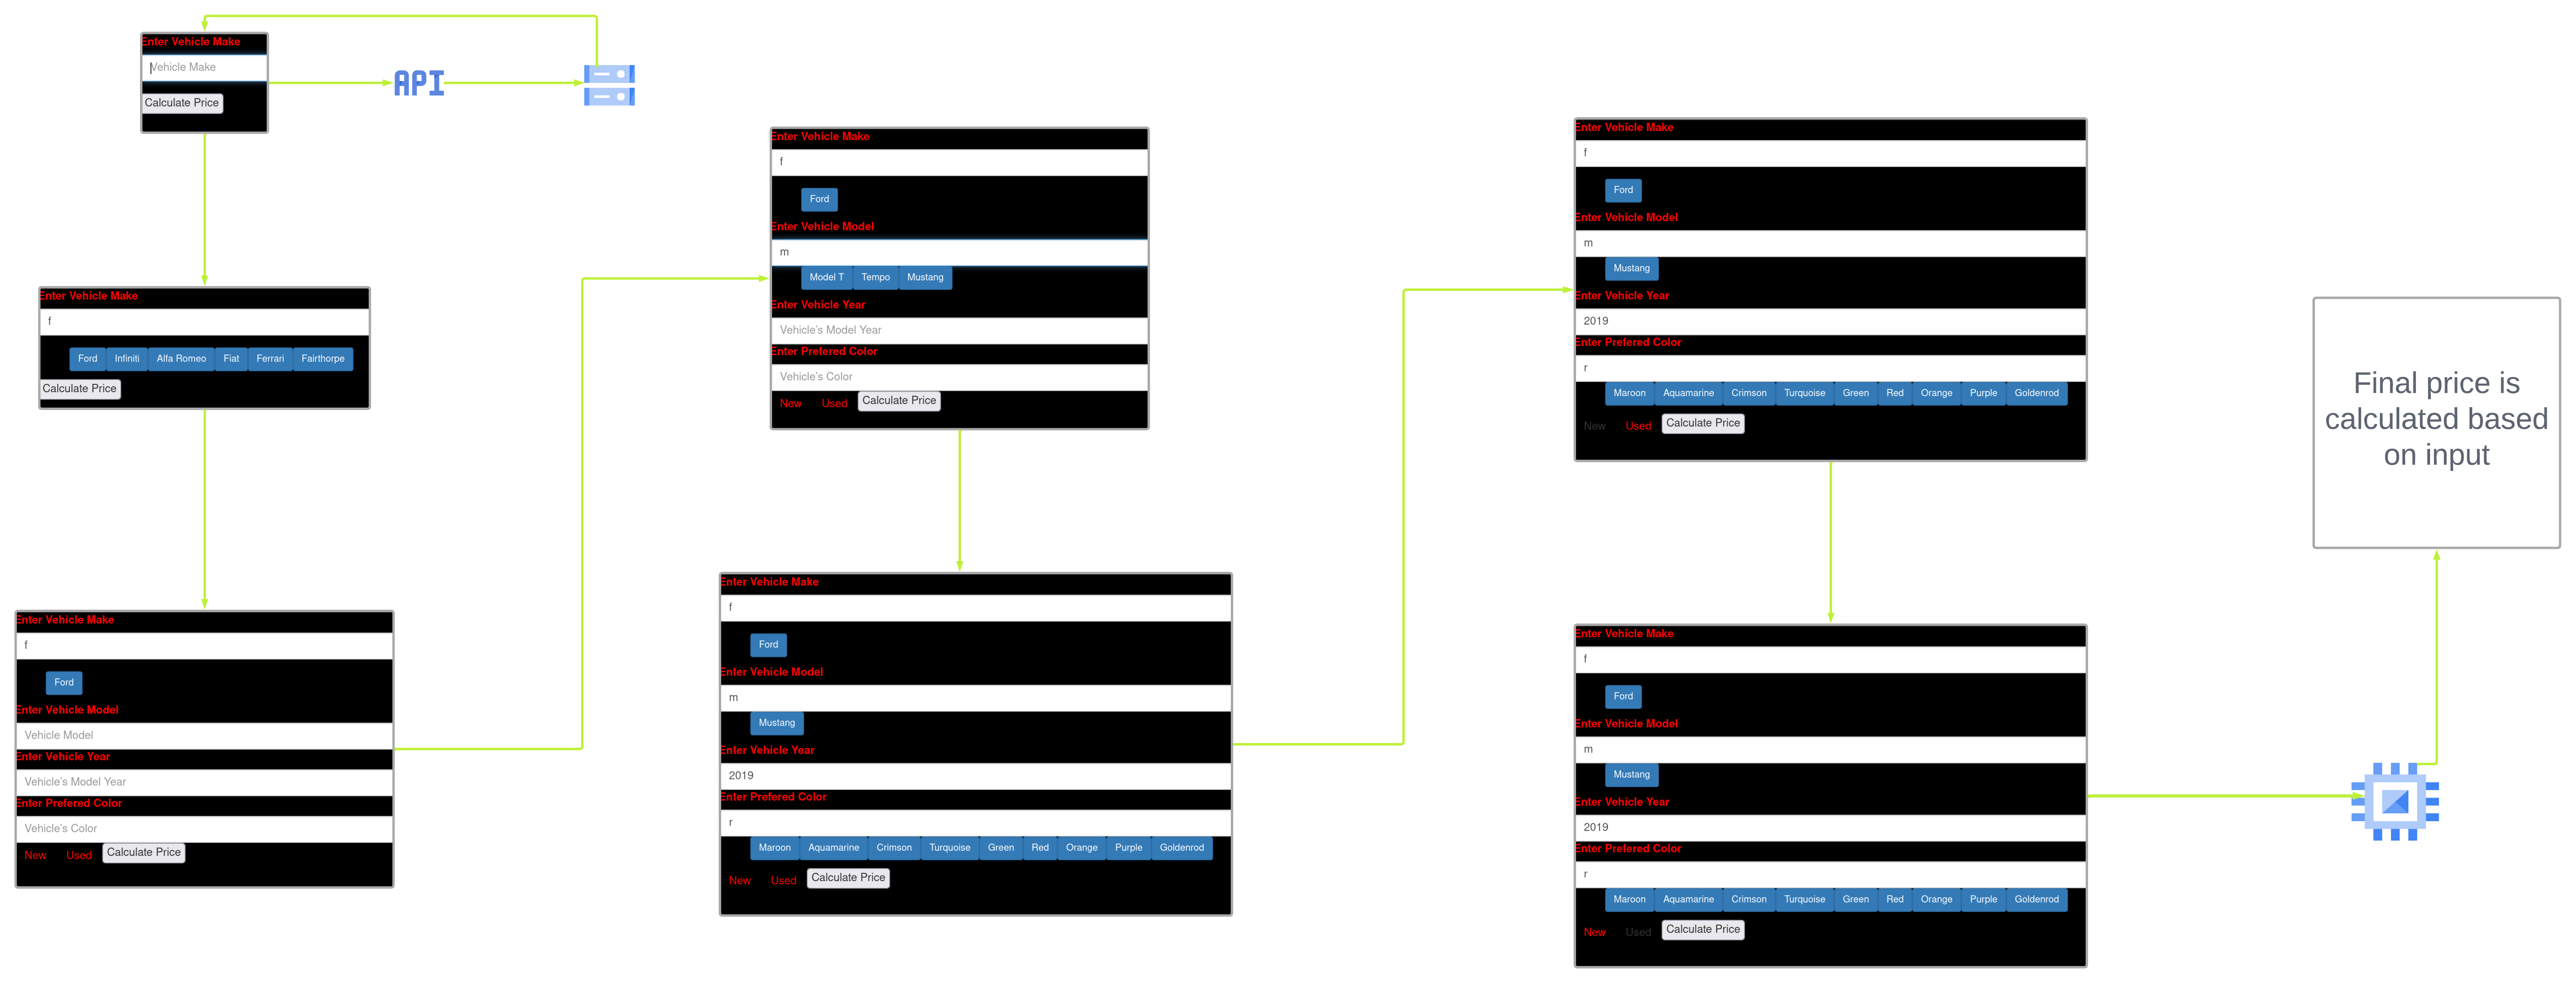
\includegraphics[scale=.078]{figures/Second Mockup.png}\\
\end{figure}
\noindent Below, Figure 7 gives an overview of how the n:point API works in conjunction with JavaScript's FETCH API.   

\begin{figure}[H]
\caption{n:point API diagram}
\centering
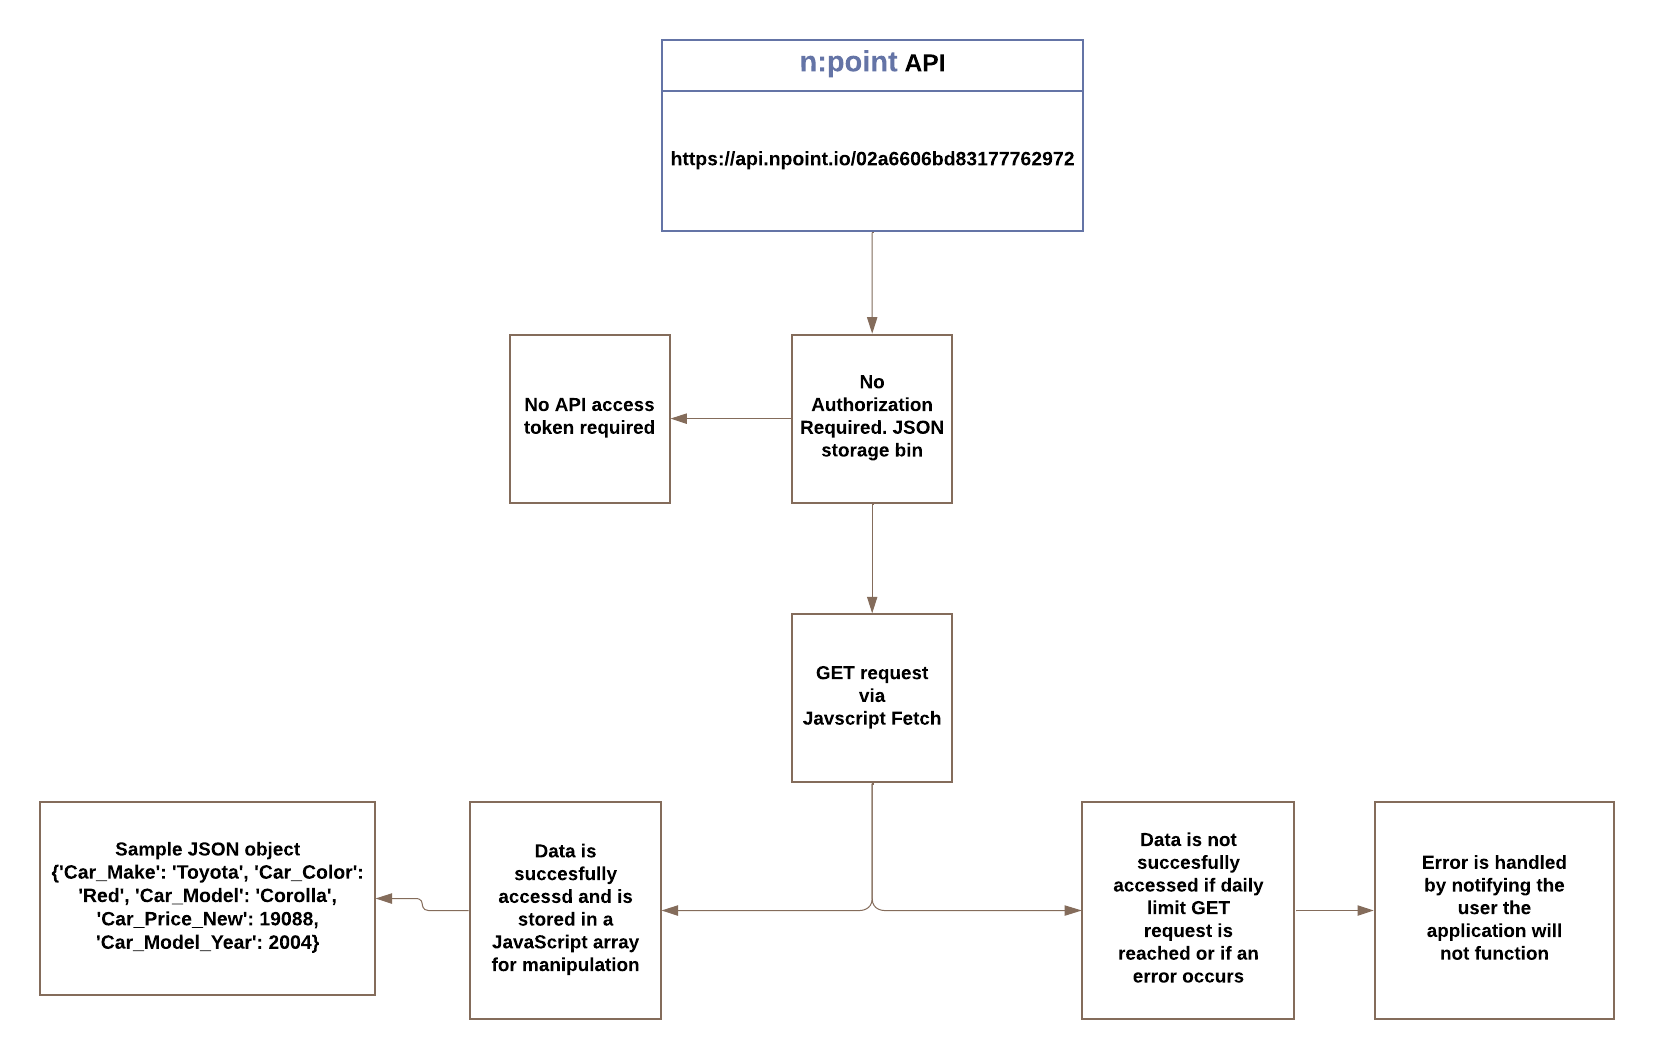
\includegraphics[scale=.25]{figures/API.png}\\
\end{figure}
\noindent To retrieve the data we first use JavaScript FETCH API to perform a GET request to n:point API where our JSON storage bin is located, since this is a storage bin we do not require an API token. API tokens are commonly used to authenticate users, to ensure that a user making a request actually has access to the requested data which is only offered to paying users \cite{dataverse.org}, in this instance, our data is publicly available. However, there are some restrictions given by n:point there can be no more than 100 requests/min per IP address or 600 requests/min per JSON bin \cite{npoint.io}. Because of this case, we must ensure that if we have reached these limitations we must handle any issues or errors derived from these limitations by notifying users that our service is down, it is highly improbable that these limits will ever be surpassed. In the case that we successfully retrieve the JSON array of objects then our application can proceed. As we can see from Figure 7 an example of one of the JSON objects that is retrieved contains the make, color, model, base price, and model year. This is an essential process that allows us to calculate a vehicle's estimated price based on user input.

\subsection{Implementation and unit testing}
As we previously mentioned in our introduction we would be using JavaScript, CSS, and HTML to build our application, we discuss our implementation and testing process. We start off with creating the first web page which is the home page, for reference on the HTML code written for this web page see Appendix \ref{subsec:B}. The home page HTML follows the basic HTML structure that every web page must have, it starts with the type of document in this case html, this is followed by a head tag that contains various metadata including the title of the web page, the favicon which is the website icon displayed by the browser, the file link to the style sheets and the meta tag that allows the web page to be responsive (mobile, desktop ready). In the body tag, we follow the structure proposed in figure 4 using Bootstrap 5 components. At the very bottom is where we provide the source of the JavaScript files we will be using, these files are delivered by a CDN and are necessary since they are a part of the Bootstrap framework. Appendix \ref{subsec:C} contains the HTML for the estimation page. Again it follows the same structure as the home page until we reach the body tag. In the body tag, there is a form tag that is the main container where the user will input their choices. Below each auto-complete supported input tag there is a div tag that is used to display the auto-completed suggestions. Appendix \ref{subsec:D} consists of the style that we added to both web pages, these styles are plainly for visuals used in the UI and are not necessarily important to discuss since they do not contribute to the overall functionality of the web page. Appendix \ref{subsec:E} is comprised of all our client-side logic that will be executed within the user's web browser. This JavaScript program consists of adding the auto-complete functionality, selecting elements from the HTML file for DOM manipulation, taking in user input for manipulation, retrieving the JSON array using FETCH API, and using all the input fields to calculate the estimated price of a vehicle. 
\begin{figure}[H]
\caption{Algorithm diagram}
\centering
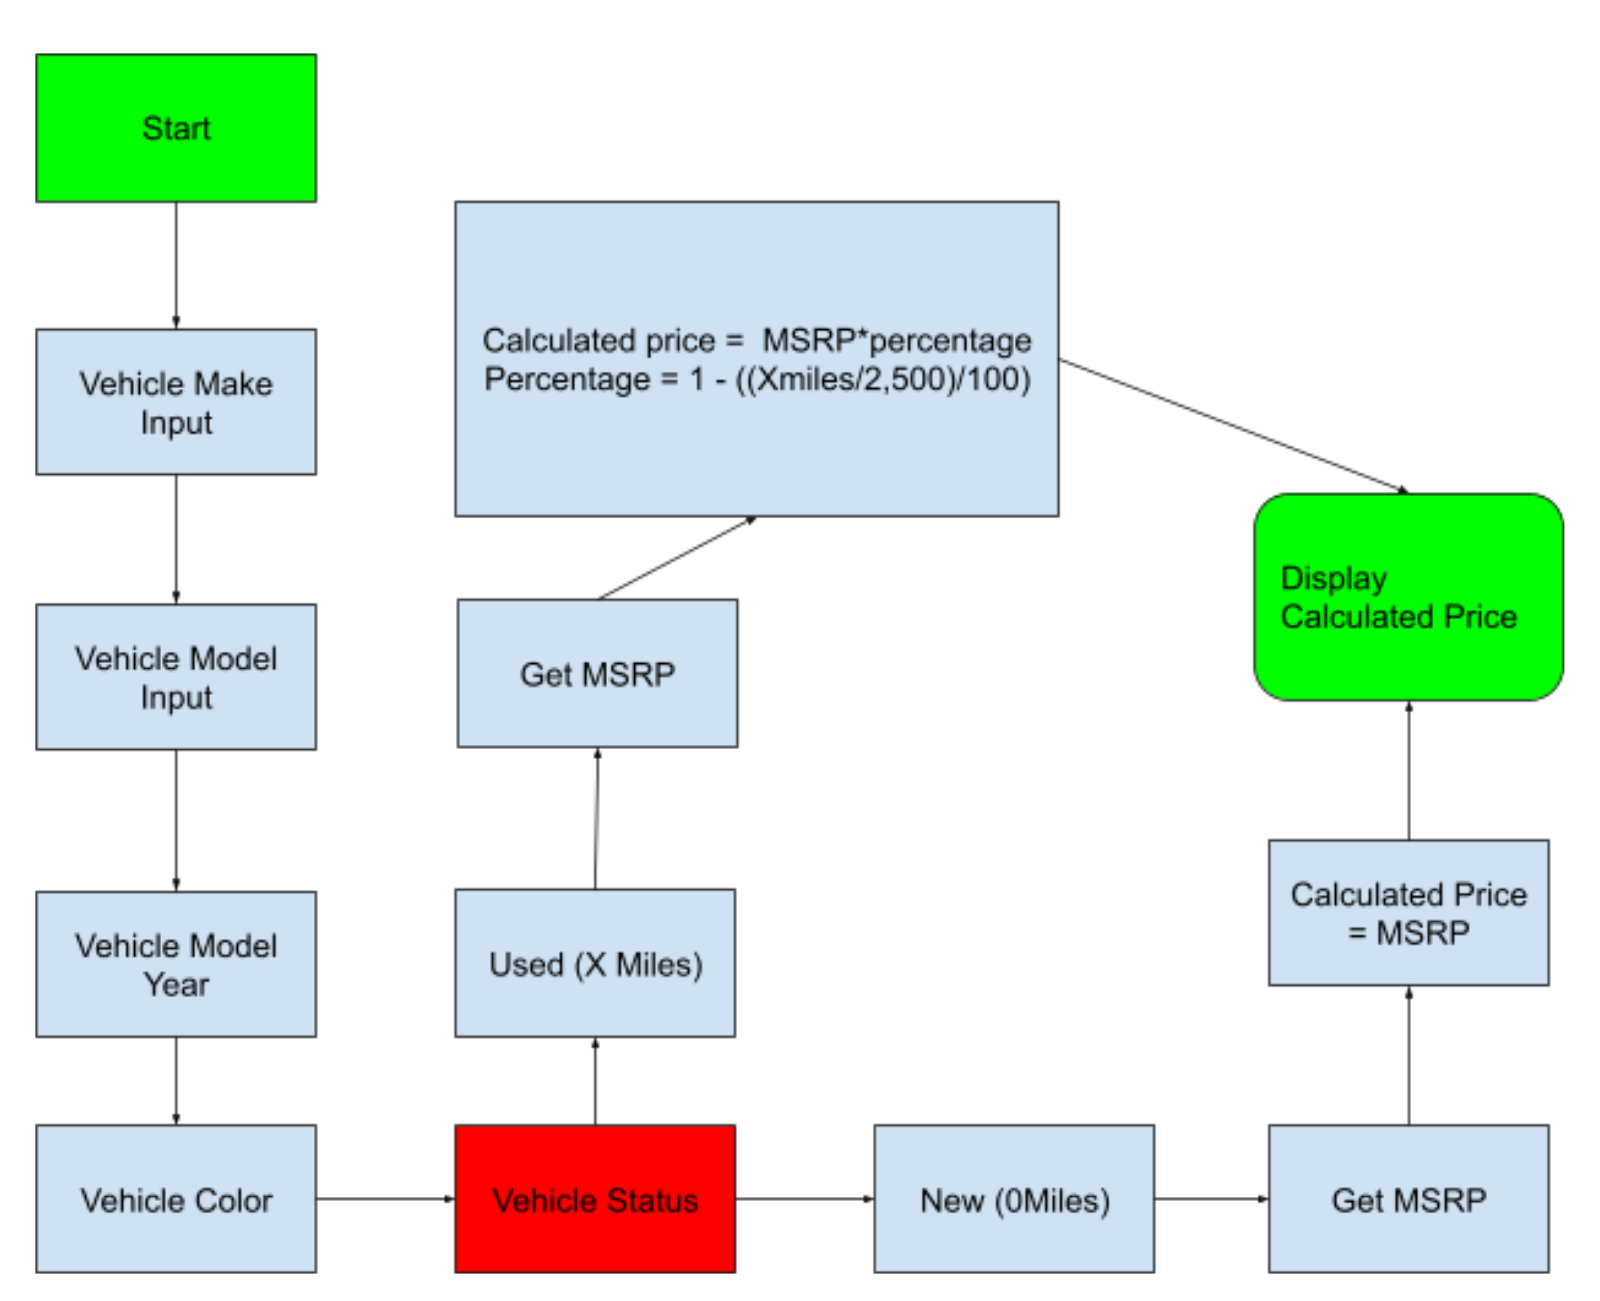
\includegraphics[scale=.25]{figures/canvas.png}\\
\end{figure}
Figure 8 describes the algorithm for computing the final price based on all input from the user. 
% --------------------
\section{Discussions and Conclusions}
\subsection{Integration and System testing}
As we have previously mentioned we decided to host our website using GitHub web pages\cite{pages.github}, this was our integration and deployment. GitHub pages are used for hosting a static website, since our website does not require a server we can use this tool for deployment, we can view our website using the following URL \url{https://lp2399.github.io/estimatecarprices.github.io/}. We now discuss our testing methods to ensure the application behaved properly. We used two cars to test out the vehicle price estimation. The first vehicle we estimated was a Red Ford Mustang from 2020, one was a new vehicle with 0 miles on the dash and the other was also a Red Ford Mustang from 2020 but this vehicle had 99,000 miles on the dash. Without calculations working we had the used car at an estimated price of \$18,119 whereas the new one would be \$29,998. The second vehicle we tested was a 2015 Green Dodge Challenger the new one with 0 miles was at an estimated price of \$22,839 whereas the used one with 69,000 miles on the dash was estimated to be worth \$16,535. Below is a set of figures from 9-12 from our unit testing the application behaved as expected.  
\begin{figure}[H]
\caption{New Mustang}
\centering
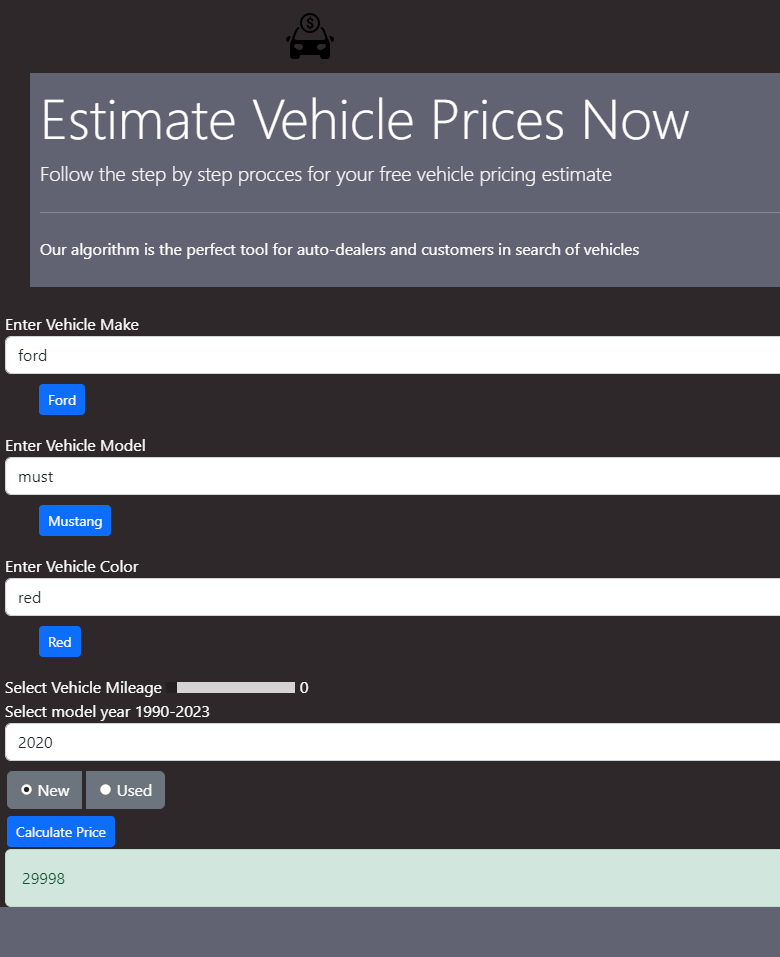
\includegraphics[scale=.6]{figures/New mustang.png}\\
\end{figure}

\begin{figure}[H]
\caption{New Challenger}
\centering
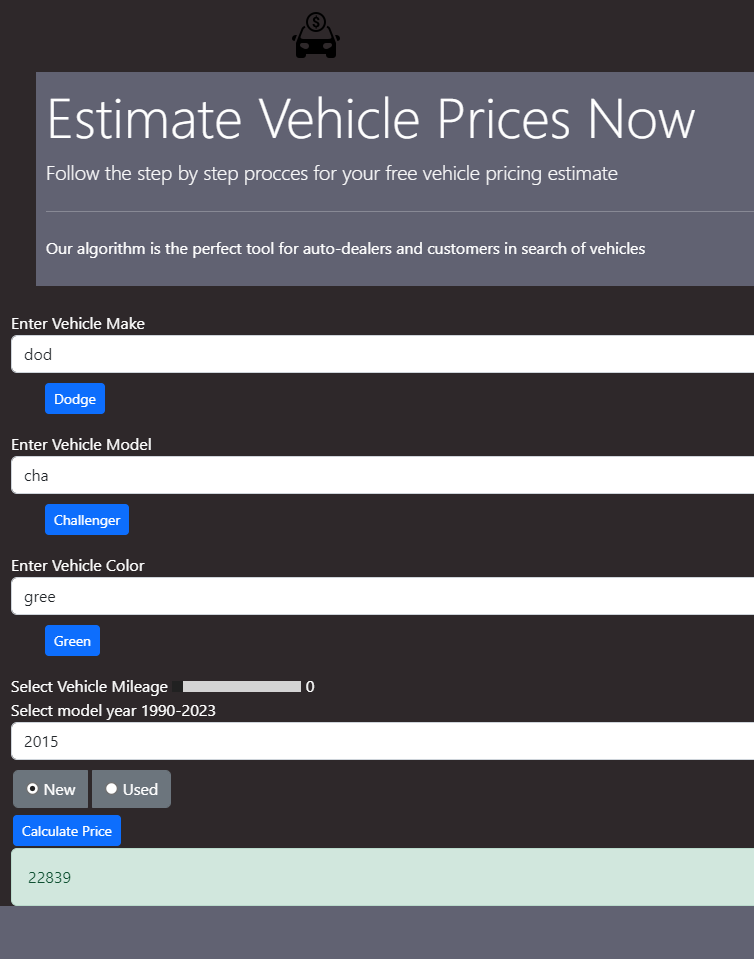
\includegraphics[scale=.6]{figures/NewChallenger.png}\\
\end{figure}

\begin{figure}[H]
\caption{Used Mustang}
\centering
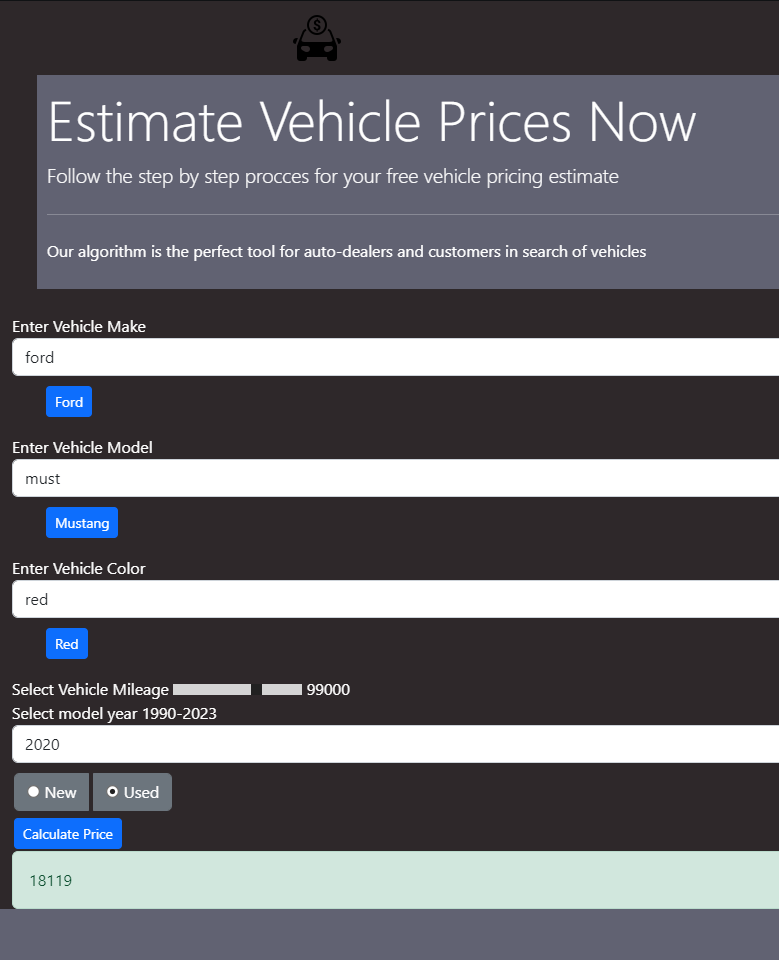
\includegraphics[scale=.6]{figures/UsedMustang.png}\\
\end{figure}

\begin{figure}[H]
\caption{Used Challenger}
\centering
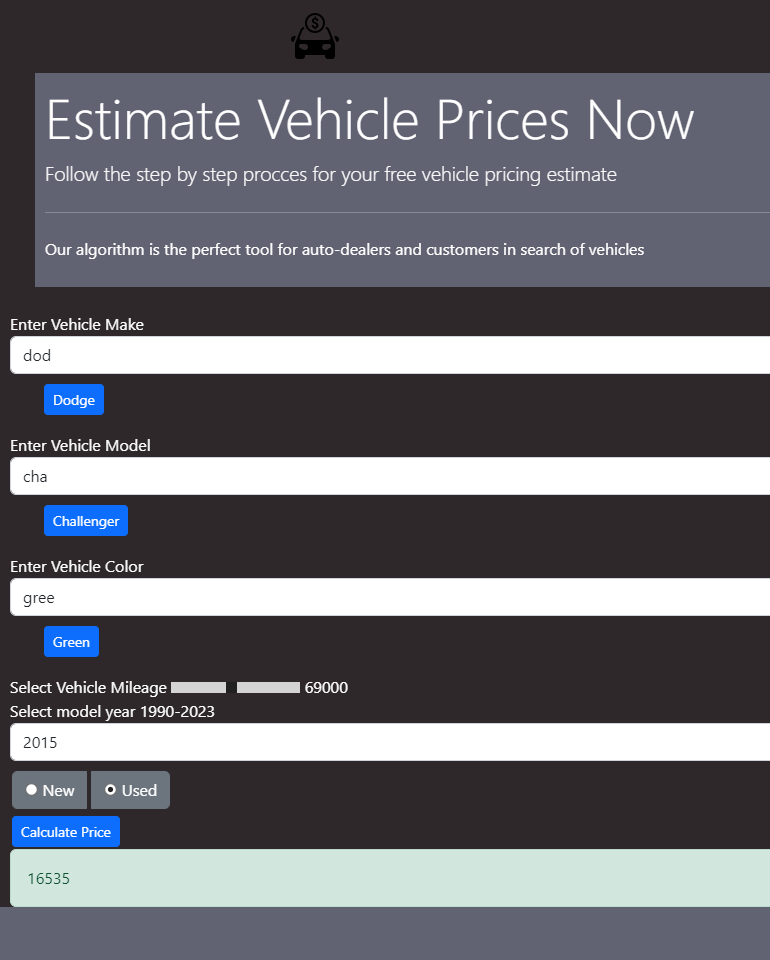
\includegraphics[scale=.6]{figures/UsedChallenger.png}\\
\end{figure}


\subsection{Operation and Maintance}
\begin{figure}[H]
\caption{Gantt Chart}
\centering
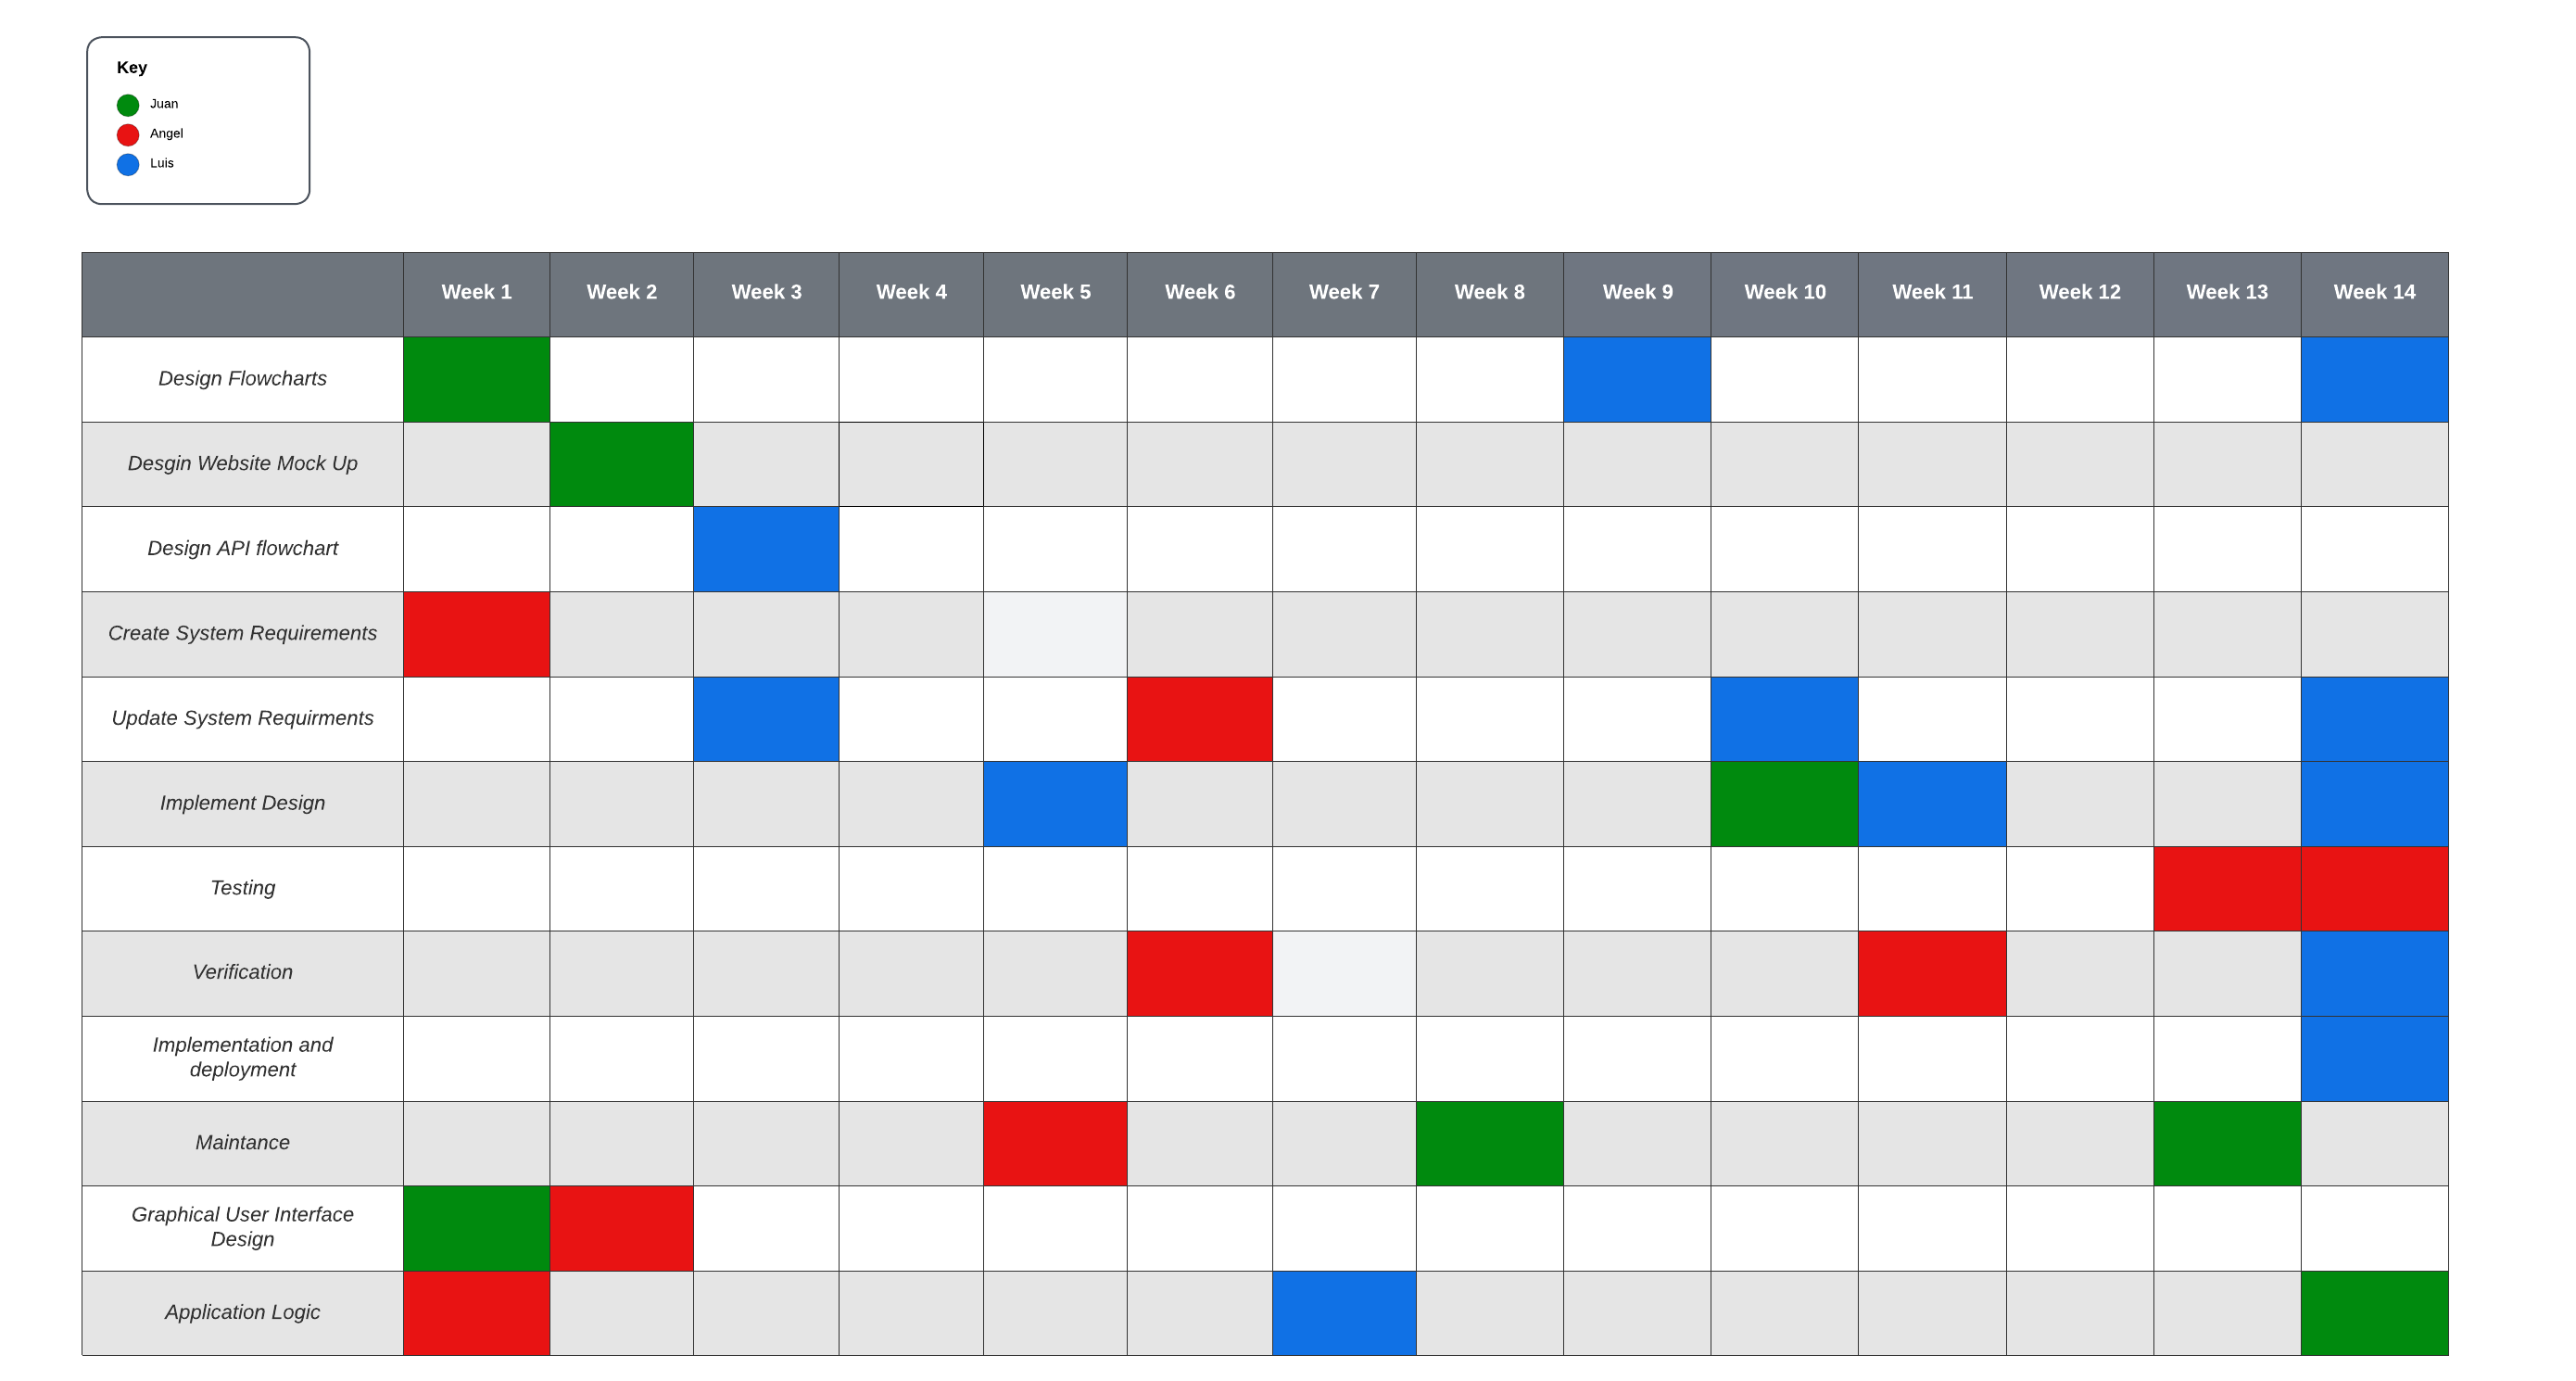
\includegraphics[scale=.199]{figures/Gantt Chart.png}\\
\end{figure}
We now discuss our work and contributions, Figure 13  demonstrates a Gantt chart, which shows the contributions each team member made. As we can see from this chart most of our work was put toward the design and implementation phases. Week 1 is where we first began the project designs and requirements, week 14 is the final week where everything was tested and completed. Each team member contributed our meeting days were Monday, and Wednesday from 12:15 PM to 1:00 PM, including the time provided during class, and Saturday from 12:00 PM to 1:00 PM. Most of our work was again done using GitHub version control, we also used messaging apps to keep ourselves on track. In the operation and maintenance section, we updated various functionality such as adding a hash table containing color keys, and prices as values. As far as maintenance goes we plan on making some additions that would have more support such as displaying images of the vehicles based on the make and model with different colors. Overall this final project allowed us to utilize various technologies and our acquired knowledge to design, implement and deploy a web application. The technologies we used of JavaScript, HTML, and CSS, with a JSON storage bin acting as our database, allowed us to have a responsive website that conformed with the requirements and is accessible from mobile and desktop devices. 
% --------------------


% %%%%%%%%%%%%%%%%%%%%%%%%%%%%%%%%%%%%%%%%%%%%%%%%%%%%%%%%%%
% %%%%%%%%%%%%%%%%%%%%%%%%%%%%%%%%%%%%%%%%%%%%%%%%%%%%%%%%%%
% REFERENCES SECTION
% %%%%%%%%%%%%%%%%%%%%%%%%%%%%%%%%%%%%%%%%%%%%%%%%%%%%%%%%%%
% %%%%%%%%%%%%%%%%%%%%%%%%%%%%%%%%%%%%%%%%%%%%%%%%%%%%%%%%%%

\bibliography{references}


\section{Appendices}
\renewcommand{\thesubsection}{\Alph{subsection}}
\subsection{System Requirements}
\label{subsec:A}

\begin{spverbatim}
Overall System Requirements

1. The system shall be comprised of two interactive web pages that should work on Chrome and Mozilla Firefox browsers for desktop and mobile. 
2. The system shall provide a home page as one of the two interactive web pages that contain an overview of the application's functionality.
4. The system shall provide a link from within the home page to the car prices estimation application page.
5. The system shall provide a link from the car prices estimation 
application page to the home page. 
6. The system shall be hosted using GitHub pages with the domain name www.estimatecarprices.github.io.
7. After the user deletes from an input field all input fields and displayed data below must be removed.
8. The user must be informed of any incorrect or unrelated input on any given input field.
9. The application should be minimalist and intuitive to use.

System Functional Requirements of the Home page.

1. The system shall upon loading display stock images that include captions describing the application and there should 
be a visible navigation bar.
2. The system shall describe the car makes that are supported by the application. 
3. The system shall provide a link at the bottom of the website that directs to the car price estimate application. 

System Functional Requirements of the car prices estimation application page.

1. The system shall upon loading provide an input box to enter vehicle make.
2. The system shall provide the user with different vehicle models depending on the vehicle make.
3. The system shall provide input fields for vehicle model year, available vehicle colors, and vehicle condition (New, Used).
4. The system should display a menu of options regarding vehicle mileage if the user selects a used vehicle.
5. The system shall then retrieve, the base price of a vehicle based on the model, year, and make. If the user selected a used vehicle the system shall accommodate the price which subtracts from the vehicle base price.
6. The system shall provide a button to calculate the final price of the vehicle based on the base price plus the color, vehicle condition, and year.
7. The system shall display the calculated price of the vehicle based on the user's input upon the user's click of a button.
\end{spverbatim}

\subsection{Home page HTML code}
\label{subsec:B}
\let\clearpage\relax
\makeatletter
\makeatother
\begin{lstlisting}[style=htmlcssjs]
<!DOCTYPE html>
<html>
    <head>
        <meta charset="UTF-8" />
        <meta name="viewport" content="width=device-width, initial-scale=1, shrink-to-fit=no" />
        <meta name="Luis Perez" content="" />
        <link type="image/png" sizes="16x16" rel="icon" href="./icons8-car-sale-16.png" />
        <meta http-equiv="X-UA-Compatible" content="ie=edge" />
        <title>Home</title>
        <link rel="stylesheet" href="style.css" />
        <link href="https://cdn.jsdelivr.net/npm/bootstrap@5.2.3/dist/css/bootstrap.min.css" rel="stylesheet" integrity="sha384-rbsA2VBKQhggwzxH7pPCaAqO46MgnOM80zW1RWuH61DGLwZJEdK2Kadq2F9CUG65" crossorigin="anonymous" />
    </head>
    <body>
        <nav class="site-header sticky-top py-1">
            <div class="container d-flex flex-column flex-md-row justify-content-between" id="navbar">
                <a class="py-2" href="index.html">
                    <img src="https://img.icons8.com/ios-filled/50/000000/car-sale.png" />
                </a>
                <a class="py-2 d-none d-md-inline-block" href="Estimate.html">Estimate</a>
            </div>
        </nav>

        <div class="container-fluid">
            <div class="carousel slide" data-bs-ride="carousel">
                <div class="carousel-indicators">
                    <button type="button" data-bs-target="#myCarousel" data-bs-slide-to="0" class="active" aria-label="Slide 1" aria-current="true"></button>
                    <button type="button" data-bs-target="#myCarousel" data-bs-slide-to="1" aria-label="Slide 2" class=""></button>
                    <button type="button" data-bs-target="#myCarousel" data-bs-slide-to="2" aria-label="Slide 3" class=""></button>
                </div>
                <div class="carousel-inner">
                    <div class="carousel-item active">
                        <img
                            class="d-block w-100 image img-fluid img-thumbnail"
                            src="https://images.unsplash.com/photo-1552519507-da3b142c6e3d?ixlib=rb-4.0.3&ixid=MnwxMjA3fDB8MHxwaG90by1wYWdlfHx8fGVufDB8fHx8&auto=format&fit=crop&w=2070&q=80"
                            alt="First slide"
                        />
                        <div class="container">
                            <div class="carousel-caption text-start">
                                <h1>Find your dream car</h1>
                                <p>Find a price estimate of your dream car based on your budject or preferences</p>
                            </div>
                        </div>
                    </div>
                    <div class="carousel-item">
                        <img class="d-block w-100 image img-fluid img-thumbnail" src="https://images.pexels.com/photos/7144243/pexels-photo-7144243.jpeg?auto=compress&cs=tinysrgb&w=1260&h=750&dpr=2" alt="Second slide" />
                        <div class="container">
                            <div class="carousel-caption">
                                <h1>Our pricing estimates are used by dealers across the country</h1>
                                <p>Each pricing estimate is guranteed to be accurate</p>
                            </div>
                        </div>
                    </div>
                    <div class="carousel-item">
                        <img class="d-block w-100 image img-fluid img-thumbnail" src="https://images.pexels.com/photos/5198239/pexels-photo-5198239.jpeg?auto=compress&cs=tinysrgb&w=1260&h=750&dpr=2" alt="Third slide" />
                        <div class="container">
                            <div class="carousel-caption text-end">
                                <h1>Our app works on any device so you can stay at home</h1>
                                <p>No need to visit a dealership simply use our app</p>
                            </div>
                        </div>
                    </div>
                </div>
                <button class="carousel-control-prev" type="button" data-bs-target="#myCarousel" data-bs-slide="prev">
                    <span class="carousel-control-prev-icon" aria-hidden="true"></span>
                    <span class="visually-hidden">Previous</span>
                </button>
                <button class="carousel-control-next" type="button" data-bs-target="#myCarousel" data-bs-slide="next">
                    <span class="carousel-control-next-icon" aria-hidden="true"></span>
                    <span class="visually-hidden">Next</span>
                </button>
            </div>
        </div>
        <div class="container-fluid">
            <div class="jumbotron">
                <h1 class="display-4">Estimate Vehicle Prices</h1>
                <p class="lead">We provide an estimate of a vehcile's price based on make, model, year, color, and condition</p>
                <hr class="my-4" />
                <p>Our algorithm is the perfect tool for auto-dealers and customers in search of vehicles</p>
            </div>
        </div>

        <div class="container-fluid">
            <div class="card text-center">
                <div class="card-body">
                    <h5 class="card-title">We provide pricing estimate for the big three</h5>
                    <p class="card-text">Ford, GM, and Chrystler are the top USA vehicle manufactures</p>
                </div>
            </div>
            <div class="card-group">
                <div class="card">
                    <img class="card-img-top img-fluid" id="img-card-1" src="https://upload.wikimedia.org/wikipedia/commons/thumb/3/3e/Ford_logo_flat.svg/2880px-Ford_logo_flat.svg.png" alt="Card image cap" />
                    <div class="card-body">
                        <h5 class="card-title">Find pricing estimates for various Ford models</h5>
                    </div>
                </div>
                <div class="card">
                    <img class="card-img-top img-fluid" id="img-card-2" src="https://upload.wikimedia.org/wikipedia/commons/thumb/d/d6/General_Motors_logo.svg/480px-General_Motors_logo.svg.png" alt="Card image cap" />
                    <div class="card-body">
                        <h5 class="card-title">Find pricing estimates for various General Motors models</h5>
                    </div>
                </div>
                <div class="card">
                    <img class="card-img-top img-fluid" id="img-card-3" src="https://upload.wikimedia.org/wikipedia/commons/a/ad/Chrysler-logo-2007-1920x1080.png" alt="Card image cap" />
                    <div class="card-body">
                        <h5 class="card-title">Find pricing estimates for various Chrystler models</h5>
                    </div>
                </div>
            </div>
            <div class="card text-center">
                <div class="card-body">
                    <h5 class="card-title">We offer pricing estimate for many other vehicle makes</h5>
                    <p class="card-text">Each make has many models to choose from</p>
                </div>
            </div>
        </div>
        <div class="container-fluid">
            <ul class="list-group">
                <li class="list-group-item">Hundai</li>
                <li class="list-group-item">Toyota</li>
                <li class="list-group-item">Honda</li>
                <li class="list-group-item">Chevrolet</li>
                <li class="list-group-item">Tesla</li>
                <li class="list-group-item">Many more</li>
            </ul>
        </div>
        <div class="container-fluid">
            <div>
                <div class="card text-center">
                    <div class="card-header">
                        Featured
                    </div>
                    <div class="card-body">
                        <h5 class="card-title">Use our algorithm to estimate the cost of a vehicle</h5>
                        <p class="card-text">Click the link below to use our app</p>
                        <a href="Estimate.html" class="btn btn-primary">Estimate Now</a>
                    </div>
                </div>
            </div>
        </div>
    </body>
    <script src="https://ajax.googleapis.com/ajax/libs/jquery/3.6.0/jquery.min.js"></script>
    <script src="https://cdn.jsdelivr.net/npm/bootstrap@5.2.3/dist/js/bootstrap.bundle.min.js"></script>
</html>
\end{lstlisting}

\subsection{Estimation page HTML code}
\label{subsec:C}
\let\clearpage\relax
\makeatletter
\makeatother
\begin{lstlisting}[style=htmlcssjs]
<!DOCTYPE html>
<html>
    <head>
        <meta charset="UTF-8" />
        <meta name="viewport" content="width=device-width, initial-scale=1, maximum-scale=1, user-scalable=no" />
        <meta name="description" content="" />
        <meta name="Luis Perez" content="" />
        <link type="image/png" sizes="16x16" rel="icon" href="./icons8-car-sale-16.png" />
        <meta http-equiv="X-UA-Compatible" content="ie=edge" />
        <title>Estimate</title>
        <link href="https://cdnjs.cloudflare.com/ajax/libs/bootstrap-datepicker/1.2.0/css/datepicker.min.css" rel="stylesheet">
        <link href="https://cdn.jsdelivr.net/npm/bootstrap@5.2.3/dist/css/bootstrap.min.css" rel="stylesheet" integrity="sha384-rbsA2VBKQhggwzxH7pPCaAqO46MgnOM80zW1RWuH61DGLwZJEdK2Kadq2F9CUG65" crossorigin="anonymous" />
        <link rel="stylesheet" href="style.css" />
        
    </head>
    <body id="Estimate-body">
        <nav class="site-header sticky-top py-1">
            <div class="container d-flex flex-column flex-md-row justify-content-between">
                <a class="py-2" href="index.html"><img src="https://img.icons8.com/ios-filled/50/000000/car-sale.png" alt="car-sale" /></a> <a class="py-2 d-none d-md-inline-block" href="index.html">Home</a>
            </div>
        </nav>
        <div class="container-fluid">
            <div class="jumbotron">
                <h1 class="display-4">Estimate Vehicle Prices Now</h1>
                <p class="lead">Follow the step by step procces for your free vehicle pricing estimate</p>
                <hr class="my-4" />
                <p>Our algorithm is the perfect tool for auto-dealers and customers in search of vehicles</p>
            </div>
        </div>
        <div class="container-fluid">
            <form autocomplete="off">
                <div class="form-group col-xs-3"><label>Enter Vehicle Make</label> <input type="text" class="form-control input-sm" id="MakeInput" placeholder="Vehicle Make" /></div>
                <div id="AutoCompletedMake"></div>
                <div class="form-group col-xs-3" id="VehicleModelSection" ><label>Enter Vehicle Model</label> <input type="text" class="form-control" id="ModelInput" placeholder="Vehicle Model" /></div>
                <div id="AutoCompletedModel"></div>
                <div class="form-group col-xs-3" id="VehicleColorSection" ><label>Enter Vehicle Color</label> <input type="text" class="form-control input-sm" placeholder="Vehicle’s Color" id="ColorInput" /></div>
                <div id="AutoCompletedColor"></div>
                <div class="form-group col-xs-3" ><label>Select Vehicle Mileage</label> <input id="SelectedMileage" type="range" value="0" min="0" step="1000" max="150000" oninput="this.nextElementSibling.value = this.value">
                <output id="SelectedMileage">0</output></div>
                <div class="form-group col-xs-3" ><label>Select model year 1990-2023</label><input type="text" class="form-control" name="datepicker" id="datepicker" /></div>   
                <div class="btn-group btn-group-toggle" data-toggle="buttons" id="NewUsedOptionButtonSection">
                    <label class="btn btn-secondary"><input type="radio" name="options" id="OptionNew" autocomplete="off" /> New</label>
                    <label class="btn btn-secondary"><input type="radio" name="options" id="OptionUsed" autocomplete="off" /> Used</label>
                </div>
                <button type="button" class="btn btn-primary btn-sm" id="CalculatePriceButton" style="display: block;">Calculate Price</button>
                <div class="alert alert-success" role="alert" id="DisplayCalculation" style="display: block;">
                </div>
            </form>
        </div>
        <script src="https://ajax.googleapis.com/ajax/libs/jquery/3.6.0/jquery.min.js"></script>
        <script src="https://cdn.jsdelivr.net/npm/bootstrap@5.2.3/dist/js/bootstrap.bundle.min.js"></script>
        <script src="https://cdnjs.cloudflare.com/ajax/libs/bootstrap-datepicker/1.2.0/js/bootstrap-datepicker.min.js"></script>
        <script src="script.js"></script>
        <script>
            $(document).ready(function(){
            $("#datepicker").datepicker({
                format: "yyyy",
                viewMode: "years", 
                minViewMode: "years",
                autoclose:true
            });   
            })
            </script>
    </body>
</html>


\end{lstlisting} 

\subsection{Styles added to both web pages code}
\label{subsec:D}
\let\clearpage\relax
\makeatletter
\makeatother
\begin{lstlisting}[style=htmlcssjs]

ul {
  list-style-type: none;
}
ul > li {
  display: inline-block;
}
.center{
  display: flex;
  justify-content: center;
  align-items: center;
  text-align: center;
}
.site-header {
  background-color: #2E282A;
  -webkit-backdrop-filter: saturate(180%) blur(20px);
  backdrop-filter: saturate(180%) blur(20px);
  top: 0;
}
.pb-1, .py-1 {
  padding-bottom: .25rem !important;
}
.pt-1, .py-1 {
  padding-top: .25rem !important;
}
.sticky-top {
  position: -webkit-sticky;
  position: sticky;
  top: 0;
  z-index: 1020;
}
.py-2{
  color: white;
}
.py-2:hover{
  color: #CD5334;
}
.jumbotron{
  background-color: #616272!important;
  color: white !important;
  background-color: #616272 !important;
  border-bottom: 25px solid #2E282A;
  border-top: transparent !important;
  border-left: 25px solid #2E282A;
  border-right: 25px solid #2E282A;
  padding: 10px;
}
.list-group-item{
  background-color: #4a434b !important;
  color: white !important;
}
.carousel{
  background-color: #616272 !important;
  border-bottom: 25px solid #2E282A;
  border-top: transparent !important;
  border-left: 25px solid #2E282A;
  border-right: 25px solid #2E282A;
}
.carousel-inner{
  border: solid 40px #6d687d;
}
.card {
  margin: 0 auto;
 /* Added */
  float: none;
 /* Added */
  margin-bottom: 10px;
 /* Added */
}
.card{
  background-color: #4a434b !important;
  color: white !important;
}
a:link {
  text-decoration: none;
}
a:visited {
  text-decoration: none;
}
a:hover {
  text-decoration: none;
}
a:active {
  text-decoration: none;
}
#img-card-2{
  max-width: 100%;
  height: 50%;
}
.card-img-top{
  height: 50%;
  width: 50%;
}
.d-block{
  opacity: .6;
}
.btn,.btn-primary, .btn-sm{
  margin-left: 2px !important;
  margin-right: 2px !important;
  margin-top: 5px !important;
  margin-bottom: 2px !important;
  display: inline;
}
.form-control{
  margin-bottom: 5px !important;
}
form{
  margin-bottom: 5px !important;
  color: white !important;
}
html{
  -webkit-touch-callout: none;
 /* iOS Safari */
  -webkit-user-select: none;
 /* Safari */
  -khtml-user-select: none;
 /* Konqueror HTML */
  -moz-user-select: none;
 /* Old versions of Firefox */
  -ms-user-select: none;
 /* Internet Explorer/Edge */
  user-select: none;
 /* Non-prefixed version, currently*/
  background-color: #616272 !important;
}
.container-fluid,body{
  background-color: #2e282a !important;
}
@media (max-width: 540px) {
  .carousel-caption > h1{
      font-size: 1vh !important;
 }
  .carousel-caption > p{
      font-size: .5vh !important;
 }
}
@media (max-width: 300px) {
  .carousel-caption > h1{
      font-size: .8vh !important;
 }
  .carousel-caption > p{
      font-size: .4vh !important;
 }
}
\end{lstlisting}

\subsection{JavaScript client-side logic code}
\label{subsec:E}
\let\clearpage\relax
\makeatletter
\makeatother
\begin{lstlisting}[style=htmlcssjs]
let jsonFetchedData = [];
const url ='https://api.npoint.io/02a6606bd83177762972'; 
let VehicleMakes = [];
let VehicleModels = [];
let VehicleBaseColors = [];
const MakeInput = document.getElementById('MakeInput');
const AutoCompleteMake = document.getElementById('AutoCompletedMake');
const ModelInput = document.getElementById('ModelInput');
const AutoCompleteModel = document.getElementById('AutoCompletedModel');
const VehicleMileageInput = document.getElementById('SelectedMileage');
const AutoCompletedColor = document.getElementById('AutoCompletedColor');
const ColorInput = document.getElementById('ColorInput');
const NewUsedOptionButtonSection = document.getElementById('NewUsedOptionButtonSection');
const CheckNewOption = document.getElementById('OptionNew');
const CheckUsedOption = document.getElementById('OptionUsed');
const CalculatePriceButton = document.getElementById('CalculatePriceButton');
const displayCalculate = document.getElementById("DisplayCalculation");
const dateInput = document.getElementById('datepicker')
let SelectedMake = '';
let SelectedModel = '';
let SelectedYear;
let SelectedColor;
let ModelYear;
let isSeletectedConditonNew;
let BasePriceNew;

function GETRequestOnlineAPI(url, callback){
  let jsonObject;
  fetch(url)
    .then(responce => responce.json())
    .then(data => jsonObject = data)
    .then(() => callback(jsonObject))
}

GETRequestOnlineAPI(url, getAPIData);


function getAPIData(Objects){
  Objects.forEach((i) => {
    jsonFetchedData.push(i);
  });
  VehicleMakes = uniqueVehicleMakeValues(jsonFetchedData);
}

function uniqueVehicleMakeValues(array) {
  return [...new Set(array.map(item => item.Car_Make))];
} 

  function AutocompleteMatch(input, options) {
    if (input == '') {
      return [];
    }
      let pattern = new RegExp(input,'gi')
      return options.filter(function(option) {
          if (option.match(pattern)) {
            return option;
          }
      });
  }

  function AutoCompleteSelector(input,options,element) {
    element.innerHTML = '';
    let button = '';
    let selected = AutocompleteMatch(input,options);
    for (i=0; i<selected.length; i++) {
        button += '<li >'+`<button type="button" class="btn btn-primary btn-sm "  id="${selected[i]}" >` + selected[i] + '</button>'+'</li>';   
    }
    element.innerHTML = `<ul id="${element.id}">` + button + '</ul>';
  }

  function DeleteNotSelectedElements(value,element){
    let SelectedOption = value.innerHTML;
    let liElements = document.getElementById(`${element.id}`).getElementsByTagName('li');
    for (var i = 0, len = liElements.length; i < len; i++ ) {
        try {
          if(liElements[i].innerText!=SelectedOption){
               element = document.getElementById(`${liElements[i].innerText}`);
               element.parentNode.removeChild(element);
          }
        }catch (error) {

            return;
          }     
     }
  }

  MakeInput.addEventListener('input',(event)=>{
    AutoCompleteSelector(event.target.value,VehicleMakes,AutoCompleteMake);
      let temp = document.getElementById(AutoCompleteMake.id).getElementsByTagName('button');
        for (let i = 0; i < temp.length; i++) {
         temp[i].addEventListener('click',(e)=>{
          DeleteNotSelectedElements(e.target,AutoCompleteMake);
          UpdateSelectedVehicleMake(e.target);
          removeVehicleModelOptions();
        })
       
      }
  });

function UpdateSelectedVehicleMake(val){
SelectedMake = val.innerText;
DisplayVehicleModelOptions();
updateDisplayCalculation();
}

function DisplayVehicleModelOptions(){
  document.getElementById("VehicleModelSection").style.display="block";
  UpdateVehicleModels();
  ModelInput.addEventListener('input',(event)=>{
    AutoCompleteSelector(event.target.value,VehicleModels,AutoCompleteModel);
      let temp = document.getElementById(AutoCompleteModel.id).getElementsByTagName('button');
        for (let i = 0; i < temp.length; i++) {
         temp[i].addEventListener('click',(e)=>{
          DeleteNotSelectedElements(e.target,AutoCompleteModel);
          UpdateSelectedVehicleModel(e.target);
        })
      }
  
  });
}

function UpdateVehicleModels(){
  VehicleModels = [];
  VehicleBaseColors = [];
  for (let i = 0; i < jsonFetchedData.length; i++) {
    if(jsonFetchedData[i].Car_Make==SelectedMake){
      VehicleModels.push(jsonFetchedData[i].Car_Model);
      VehicleBaseColors.push(jsonFetchedData[i].Car_Color);
    }; 
  }
  VehicleModels = [...new Set(VehicleModels)];
  VehicleBaseColors = ["White", "Black", "Gray", "Silver", "Blue", "Red", "Brown", "Green", "Orange", "Beige", "Purple", "Gold", "Yellow"];
  updateDisplayCalculation();
}
function removeVehicleModelOptions(){
  MakeInput.addEventListener('input',()=>{
    document.getElementById("VehicleModelSection").style.display="none";;
  });
  UpdateVehicleModels();
}

  ColorInput.addEventListener('input',(event)=>{
    AutoCompleteSelector(event.target.value,VehicleBaseColors,AutoCompletedColor);
      let temp = document.getElementById(AutoCompletedColor.id).getElementsByTagName('button');
        for (let i = 0; i < temp.length; i++) {
         temp[i].addEventListener('click',(e)=>{
          DeleteNotSelectedElements(e.target,AutoCompletedColor);
          UpdateSelectedColor(e.target);
        })
      }
  });

function UpdateSelectedVehicleModel(val){
  SelectedModel = val.innerText;
  updateDisplayCalculation();
  }

function UpdateBaseVehicleYear(val){
  ModelYear= val.innerText;
  }
function UpdateSelectedColor(val){
  SelectedColor = val.innerText;
}  


CheckNewOption.addEventListener('click',(event)=>{
  if(event.target.value =='ON'){
    isSeletectedConditonNew = true;  
  }
})

CheckUsedOption.addEventListener('click',(event)=>{
  if(event.target.value =='ON'){
    isSeletectedConditonNew = false;  
  }
})


CalculatePriceButton.addEventListener('click',(event)=>{
  CalculateFinalPrice();
})

function updateDisplayCalculation(){
  displayCalculate.innerHTML = '';
}

function CalculateFinalPrice(){
  displayCalculate.innerHTML = "";
  let a = AutoCompleteMake.childNodes[0].innerText;
  let b = AutoCompleteModel.childNodes[0].innerText;
  let c = AutoCompletedColor.childNodes[0].innerText;
  let colorsHashtable = new Map();
  colorsHashtable.set("White", 0);
  colorsHashtable.set("Black", 0);
  colorsHashtable.set("Gray", 300);
  colorsHashtable.set("Silver", 1000);
  colorsHashtable.set("Blue", 1000);
  colorsHashtable.set("Red", 300);
  colorsHashtable.set("Brown", 600);
  colorsHashtable.set("Green", 600);
  colorsHashtable.set("Orange", 500);
  colorsHashtable.set("Beige", 1000);
  colorsHashtable.set("Purple", 100);
  colorsHashtable.set("Gold", 2000);
  colorsHashtable.set("Yellow", 200);

  let temp = [];
  for (let i = 0; i < jsonFetchedData.length; i++) {
      let j =  jsonFetchedData[i];
      if(j.Car_Make==a && j.Car_Model==b){
        temp.push(j)
      }
  }

  let summation = 0;
  for(let i = 0; i < temp.length; i++) {
      summation += temp[i].Car_Price_New;
  }

  let MSRP =  (summation / temp.length)+colorsHashtable.get(String(c));// base price 



  if(isSeletectedConditonNew){
    VehicleMileageInput.value= 0;
  }
  
  displayCalculate.innerHTML = Math.round(MSRP * (1-((VehicleMileageInput.value/2500)/100)));
}
\end{lstlisting} 

\subsection{Additional Icons, and Images Used for Visuals Throughout the Entire Project and GitHub repository}
\label{subsec:F}
\begin{lstlisting}[breaklines]
https://github.com/lp2399/Software_Engineering_Project/blob/main/images_sources.txt
https://github.com/lp2399/Software_Engineering_Project
\end{lstlisting}

\newpage
\end{document}